\cotefile{72}
\scanpage{35}
\margin{?}
D'ailleurs, si $N=2$, $\exists!$ \deleted{\unsure{quadrique}}\inserted{conique} $Q\subset X$ \unsure{invariante} par $\varphi^+$, et elle est $=$ invariante par $\varphi$.

[\unsure{Peut-être} faux. Il \unsure{en} \unsure{donne} \unsure{un} \unsure{pr.} \unsure{ch.} \deleted{\unsure{formes quadratiques}}\inserted{\unsure{hyp. pour exclure les}} invariantes \unsure{...}]
\mspage{34}

\scanpage{36}
\unsure{Supposons} les $\beta_i\inserted{=\alpha_i+2}$ inv.
\[
\begin{array}{rcl}
\text{forme sur }\unsure{\mathcal L}(a_{i-1},a_i,a_{i+1})\text{ lisse}
&\Longleftrightarrow&\alpha_{i-1}+\alpha_i\quad\text{inv.}\\
\text{forme sur }\unsure{\mathcal L}(a_{i-1},a_i)\text{ lisse}
&\Longleftrightarrow&2-\alpha_{i-1}\quad\text{inv.}\\
\longrightarrow\quad\unsure{\mathcal L}(a_i,a_{i+1})\text{ lisse}
&\Longleftrightarrow&2-\alpha_i\quad\text{inv.}
\end{array}
\]
\deleted{$\unsure{\alpha_i}$}
\figure{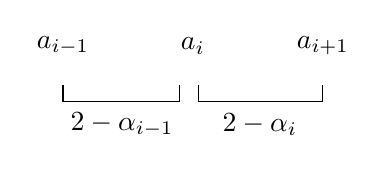
\begin{tikzpicture}[x=1cm,y=1cm]
\node at (0,0.45) {$a_{i-1}$}; \node at (1.65,0.45) {$a_i$}; \node at (3.3,0.45) {$a_{i+1}$};
\draw (0,-0.05)--(0,-0.25)--(1.48,-0.25)--(1.48,-0.05);
\draw (1.72,-0.05)--(1.72,-0.25)--(3.3,-0.25)--(3.3,-0.05);
\node at (.75,-.55) {$2-\unsure{\alpha_{i-1}}$}; \node at (2.5,-.55) {$2-\alpha_i$};
\end{tikzpicture}}
$\alpha_i\ne2$. \unsure{pas} de val. propres $1$
\[
\alpha_{\unsure{i-1}}\ne2.
\]
\deleted{\unsure{Ret.}} Si
\margin{Sur $1\le i\unsure{\leq|<}n-1$}
\diagram{\begin{tikzcd}[ampersand replacement=\&,column sep=large,row sep=small]
\& |[draw,rounded corners]| \text{donc car. }\ne2!\\
\left.\begin{array}{l}
\beta_0,\ldots,\beta_{n-1}\quad\text{inv.}\\
2(\alpha_{i-1}+\alpha_i)\quad\text{inv.}\\
\alpha_{i-1}-2,\ \alpha_i-2\quad\text{inv.}
\end{array}\right\}\arrow[ur] \&
\end{tikzcd}}
alors $\tau_i$ se reconstruit à partir des
$\underset{\substack{\Vert\\\tau_{i-1}\tau_i}}{\rho_{i-1}},\
\underset{\substack{\Vert\\\tau_i\tau_{i+1}}}{\rho_i}$,
donc aussi
\[
\tau_{i-1}=\rho_{i-1}\tau_i,\qquad
\tau_{i+1}=\tau_i\rho_i.
\]
\margin{\uline{dans $V,f$}\quad $C=\mathbb P(V)\unsure{\setminus}Q$\quad $(n\ge2)$}
$\tau_i=$ \deleted{\unsure{sym.}} réflexion associée à la \uline{direction}
\[
\begin{aligned}
\left(
\underbrace{V^{\rho_{i-1}}}_{\substack{\deleted{\unsure{\subset}}\Vert\\\{a_{i-1},a_i\}^{\perp}}}
+
\underbrace{V^{\rho_i}}_{\substack{\Vert\\\{a_i,a_{i+1}\}^{\perp}}}
\right)^\perp
&=\{a_{i-1},a_i\}^{\perp\perp}\cap\{a_i,a_{i+1}\}^{\perp\perp}\\
&=\unsure{\mathcal L}(a_{i-1},a_i)\cap\unsure{\mathcal L}(a_i,a_{i+1}).
\end{aligned}
\]
\[
\alpha_i=\frac{(a_i,a_{i+1})^2}{f(a_i)f(a_{i+1})}
=4\cos^2\theta_i\cdot\deleted{\unsure{2\cos2}}.
\]
\[
\beta_i=\alpha_i+2
=2\bigl(\underbrace{2\cos^2\theta_i+1}_{\deleted{\unsure{2}}\cos2\theta_i}\bigr)
=4\cos2\theta_i.
\]
\mspage{35}

\scanpage{37}
\[
\unsure{\mathcal U}_{\rho}\simeq
\operatorname{Aut}\bigl(\unsure{\mathcal G|\mathcal X},(\tau_{\unsure{a|i}})\bigr)
\]
\mspage{36}

\scanpage{38}
Soit $\rho\in\Gamma(S,\mathcal O_S)$, $U_\rho\subset E^1_S$ formé des $\lambda$ tels que
$1+\lambda\rho$ inversible i.e.
\[
U_\rho=\uline{\operatorname{Spec}}\ \mathcal O_S[T]_{(1+\rho T)}
\]
prenons la multiplication
\[
\unsure{(}\lambda *_\rho\lambda'=\lambda+\lambda'+\lambda\lambda'\rho
\]
de sorte que $U_\rho$ est un schéma en groupes
\inserted{(\unsure{Assoc.} comm. \unsure{él. unit.} $\unsure{1}$)}, et
\diagram{\begin{tikzcd}[ampersand replacement=\&,column sep=large,row sep=small]
\lambda \arrow[r,maps to,no head] \& 1+\lambda\rho\\
U_\rho \arrow[r,no head] \& \mathbb G_m
\end{tikzcd}}
est un hom. de groupes, qui est un iso. sss $\rho$ inversible.

Considérons un hyperpolyèdre régulier \unsure{ponctué|pointé} épinglé sur $S$, de dim. $n$,
\inserted{(\unsure{conn.})}
correspondant à des invariants $\mu_i$ $(0\le i\le n)$ et $\beta_i$
$(0\le i\le n-1)$ [avec $\mu_i+1$ inv. $0\le i\le n$).
\unsure{Soit}
\deleted{$\rho=\unsure{\mathbb L}_{n+1}(\mu_0,\lambda_0,\ldots,\unsure{\lambda_{n-1}},\mu_n)$}
\[
\unsure{=}\qquad
\rho=\unsure{\mathbb L}_{n+1}(\mu_0,\lambda_0,\ldots,\lambda_{n-1},\mu_n)
=\langle\Pi,\Pi'\rangle
\]
\mspage{37}

\scanpage{39}
Donc $U_\rho$ opère \inserted{\uline{fidèlement}} sur $\mathcal E,\mathcal E'$ par
\[
\left\{
\begin{aligned}
u_\lambda^{\mathcal E}&=\operatorname{id}+\lambda\Pi'\otimes\Pi\\
u_\lambda^{\mathcal E'}&=\operatorname{id}+\lambda\Pi'\otimes\Pi
\end{aligned}\right.
\]
(opérations \deleted{\unsure{contragrédientes}}\inserted{transposées} l'une de l'autre)
Comme $\Pi,\Pi'$ invariants sous les $\tau_i$, donc sous les
$\varphi^{\mathcal E}(s)$, $\varphi_{\unsure{s}}^{\mathcal E'}(s)$
$(s\in\unsure{\mathfrak G_n})$, on trouve
\[
\unsure{(\alpha')}\qquad
\diagram{\begin{tikzcd}[ampersand replacement=\&]
U_\rho\arrow[r] \& \uline{\operatorname{Aut}}(\mathcal E,\varphi^{\mathcal E})
\end{tikzcd}}
\]
\[
\unsure{(\alpha)}\qquad
\diagram{\begin{tikzcd}[ampersand replacement=\&]
U_\rho\arrow[r] \& \uline{\operatorname{Aut}}(X,\varphi^X)
\end{tikzcd}}
\]
et de $=$ sur $\mathcal E'$. On obtient en fait, en \unsure{adjoignant} les scalaires
\[
\unsure{(\alpha\alpha)}\qquad
\diagram{\begin{tikzcd}[ampersand replacement=\&,column sep=large]
\mathbb G_m\times U_\rho\arrow[rr]\arrow[dr,bend right]\& \&
\operatorname{Aut}(\mathcal E,\varphi^{\mathcal E})\\
\&\mathbb G_m\arrow[ur,"\text{opère par \unsure{homothéties}}"']\&
\end{tikzcd}}
\]
dont $\unsure{\alpha}$ est déduit en passant au quotient. On trouve

\uline{Thm}\quad $\unsure{\alpha}$ et $\unsure{(\alpha\alpha)}$ sont des iso.

\margin{\figure{\begin{tikzpicture}\draw (0,0)--(0,-1.7);\end{tikzpicture}}}
De plus, si $D_0=(H_1\cap\cdots\cap H_n)$,
$\uline{D_0^{**}}=D_0\setminus\{c,d\}$, où
$\unsure{\{d\}}=D_0\cap C$ (qui est une section de $X$ sur $S$) on a que
\mspage{38}

\scanpage{40}
$U_\rho$ opère (\unsure{sans unité}) sur $D_0$ et $D_0^{**}$,
et que $D_0^{**}$ est un \uline{torseur} sous $U_\rho$
(trivialisé par $\unsure{b_{0\ldots n}}$).

\figure{\begin{tikzpicture}\draw (0,0)--(2,0);\end{tikzpicture}}

Supposons maintenant les $\mu_i=\unsure{2}$ de sorte qu'on a une forme quadratique
\uline{inv.} canonique $f$ sur $\mathcal E$, unique par la condition
\[
f(a_{\unsure{-1}})=0,\qquad f(e_0)=1,
\]
\deleted{\unsure{Je ai}}
d'où $Q\subset X=\mathbb P^{\unsure{\vee}}(\mathcal E)$.

On sait que la \unsure{ps. réfle}
$\operatorname{id}+\underbrace{\unsure{\lambda}\Pi'\otimes\Pi}_{\Pi'\otimes\lambda\Pi}$
est \deleted{\unsure{une}} orthogonale sss l'opération \unsure{corr.}
dans $X$ conserve $Q$, et ceci signifie que
\[
\lambda\,\deleted{\unsure{\Psi}}\inserted{f}(\lambda\Pi)\Pi'
+\Psi(\lambda\Pi)=0\quad\text{i.e.}
\]
\[
\lambda\left[
\lambda\underbrace{f(\Pi)}_{\inserted{-\widetilde\sigma\widetilde\rho}}\Pi'
+\underbrace{\Psi(\Pi)}_{\inserted{-\sigma\Pi'}}
\right]=0\qquad\text{i.e.}
\]
\deleted{$\unsure{\lambda\rho\Pi'+\Psi}$}
\[
\unsure{(\alpha b)}\qquad
\lambda(\sigma+\lambda\widetilde\sigma\widetilde\rho)=0
\]
\mspage{39}

\scanpage{41}
1) Cas $n$ pair, $\rho=2\widetilde\rho$, $\sigma=\widetilde\sigma$, l'équation s'écrit
\[
\lambda\sigma(1+\deleted{\unsure{2}}\lambda\widetilde\rho)=0
\]
Si $\sigma$ \deleted{\unsure{est}}\inserted{et $\widetilde\rho$} inversibles,
la seule solution \uline{inversible}
(\inserted{i.e.} correspondant à une section de $U_\rho$ partout $\ne1$)
est donnée par
\[
\lambda=-\frac{1}{\deleted{\unsure{2}}\widetilde\rho}
\qquad\text{d'où}\qquad
\underbrace{u=\operatorname{id}-\frac{1}{\deleted{\unsure{2}}\unsure{\widetilde\rho}}\Pi'\otimes\Pi}
_{\uline{\text{antipodisme}}}.
\]
\deleted{Si $\uline{\sigma=0}$ $U_\rho$ invarie $f$, on a que}
D'autre part conditions équivalentes
\deleted{\unsure{on a}}
\diagram{\begin{tikzcd}[ampersand replacement=\&,column sep=0pt,row sep=small]
\& \text{b) }U_\rho\text{ invarie }f^{\mathcal E}\\
\& \text{\unsure{c)} }U_\rho\text{ invarie }Q_X^{\deleted{\unsure{\mathcal E}}}\\
\& \text{a) }\sigma=0\arrow[uu,bend left=65,start anchor=west,end anchor=west]
\end{tikzcd}}

Enfin, si $\widetilde\rho=0$, \deleted{\unsure{alors}}\inserted{ces} conditions équivalentes encore à la suivante
\deleted{$\unsure{\text{c) }\sigma=0}$}

d) $\exists$ loc. section \deleted{\unsure{différente}} de $U_\rho$ partout
$\ne1$, qui invarie $f^{\mathcal E}$.
\deleted{(\unsure{qui invarie} $Q_X$)}
\inserted{(\unsure{ou aussi} $Q_X$)}.

\deleted{\unsure{partout} $\unsure{\ne1}$}
\mspage{40}

\scanpage{42}
2) Cas $n$ impair $\rho=\widetilde\rho$, $\sigma=2\widetilde\sigma$,
l'équation s'écrit
\[
\lambda\widetilde\sigma(2+\lambda\rho)=0.
\]
Donc si $\inserted{\sigma}(=2\widetilde\sigma)$ et $\rho\inserted{(=\widetilde\rho)}$ inv.,
\deleted{la seule} $\exists!$ section $u$ de $U_\rho$, partout $\ne1$,
\deleted{telle} qui invarie $f$, --- ce qui revient au $=$, qui invarie $Q$ --- savoir
\[
\underbrace{u=\operatorname{id}-\frac{2}{\rho}\Pi'\otimes\Pi}_{\text{antipodisme}}
\]
\margin{\uline{NB} Si $\widetilde\sigma$ inv. et non $\sigma$ (\unsure{p. ex.} en car. $2$)
on a \unsure{donc} bien unique solution en $\lambda$, \unsure{savoir que}
$\lambda=-\frac{2}{\rho}$, mais celle-ci peut être nulle en certains pts.
Donner un énoncé commun aux cas $1^\circ)$ et $2^\circ)$ \uline{en termes de}
\figure{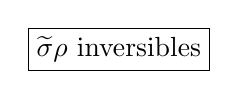
\begin{tikzpicture}
\node[draw,inner sep=3pt] {$\unsure{\widetilde\sigma\rho}$ inversibles};
\end{tikzpicture}}}

D'autre part, conditions \unsure{équivalentes}\deleted{\unsure{alors}}
\deleted{$\unsure{\sigma}$}

a) $2\widetilde\sigma=\sigma=0$ et
$\widetilde\sigma\rho\inserted{(=\unsure{\sigma\widetilde\rho})}=0$

[\uline{NB} Si $2$ inv., ceci équivaut à $\sigma=0$; si $2=0$,
ceci équivaut à $\widetilde\sigma\rho=0$]

b) $U_\rho$ invarie $f^{\mathcal E}$

c) $U_\rho$ \unsure{---} $Q_X$
\margin{\unsure{i.e.}}

Si \deleted{de plus} $\rho=0$, ces conditions équivalent aussi à :

d) $\exists$ \inserted{loc.} section de $U_\rho$ partout $\ne1$ qui
invarie $f^{\mathcal E}$ (ou encore, $Q_X$)
\mspage{41}

\scanpage{43}
[\uline{Ex} $n=1$, $\rho=4-\beta=2-\alpha$, $\sigma=\deleted{\unsure{alors}}2$,
$\widetilde\sigma=1$. Donc

\deleted{\unsure{Par}} $1^\circ)$ si $\deleted{\unsure{2}}\rho$ inv.
\inserted{i.e. $U_\rho\simeq\mathbb G_m$},
\deleted{alors} $\exists!$ $u\in U_{\rho=2-\alpha}$ partout $\ne1$,
telle que $u$ invarie $f^{\mathcal E}$ (--- ce qui revient au $=$,
\deleted{$\unsure{Q_X}$} la conique $Q_X$)
savoir l'antipodisme, qui est l'unique section $u$ telle que
$u^2=1$, $u_s\ne1$ $\forall s\in S$.

$2^\circ)$ Conditions équivalentes

a) $\rho=0$ et \deleted{\unsure{sur}} $S$ de car $2$ $(2.1_S=0)$

b) $U_\rho$ invarie $f^{\mathcal E}$

c) $U_\rho$ --- $Q_X$

d) $\rho=0$ et $\exists$ loc. section partout $\ne1$,
qui invarie $f^{\mathcal E}$ (ou encore, $Q_X$). ]

\figure{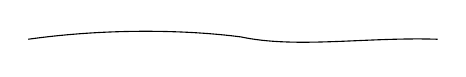
\begin{tikzpicture}
\draw (0,0)..controls(1,.14)and(2,.12)..(2.7,.03)..controls(3.4,-.12)and(4.3,.03)..(5.2,0);
\end{tikzpicture}}

\uline{Proposition}\quad 1) Si $\sigma\widetilde\rho$ inversible,
$\exists!$ section $u$ de $U_\rho$, partout $\ne1$, qui invarie $f^{\mathcal E}$
i.e. $Q_X$, savoir l'antipodisme.

2) Conditions équivalentes

a) $\sigma=0$ et $\widetilde\sigma\widetilde\rho=0$
\margin{(cette dernière condition conséquence de la première si $n$ pair ou $2$ inv.)}

b) $U_\rho$ invarie $f^{\deleted{\unsure{\mathcal E}}\inserted{\mathcal E}}$

c) $U_\rho$ invarie $Q_X$

\margin{\unsure{?}}
d) (\uuline{Si $\widetilde\sigma\widetilde\rho=0$})
$\exists$ loc. section de $U_\rho$ partout $\ne1$, qui invarie $f^{\mathcal E}$
(ou $Q_X$)
\mspage{42}

\scanpage{44}
Calculs de discriminant

\unsure{etc}
\mspage{43}

\scanpage{45}
\[
\left\{
\begin{aligned}
f(s_i)&=0\\
\varphi(s_i,s_j)&=-(\alpha_0+2)\cdots(\alpha_{i-1}+2)
\qquad 0\leq i<j\leq n+1
\end{aligned}
\right.
\]
$f$ caractérisée par les conditions
\[
\begin{aligned}
\text{a)}\;&f\ \text{inv. par les }\tau_i\\
\text{b)}\;&f(s_0)=0\quad
(\Longleftrightarrow f\ \text{nulle sur les sommets \unsure{géom.} de }\Pi\\
\text{c)}\;&f(a_0)=1\quad
(\Longleftrightarrow \deleted{\unsure{\text{les}}}\ \text{vecteurs arêtes sont unitaires})
\end{aligned}
\]
\[
f(a_i)=(\alpha_0+2)\cdots(\alpha_{i-1}+2)\qquad0\leq i\leq n
\]
\[
\varphi(a_i,a_j)=0\qquad0\leq i<j\leq n,\quad i,j\ \text{non conséc.}
\]
\[
\varphi(a_i,a_{i+1})=-(\alpha_0+2)\cdots(\alpha_i+2)
\]
\[
\varphi(s_0,a_i)=0\qquad1\leq i\leq n
\]
\[
\varphi(s_0,a_0)=-1
\]
\[
\varphi(s_j,a_i)=0\qquad0\leq j<i\leq n,\quad
\deleted{\unsure{i<j+1}}
\]
\[
\varphi(s_j,a_{j\deleted{\unsure{+1}}})
=-(\alpha_0+2)\cdots(\alpha_{j-1}+2)
\qquad0\leq j\leq n
\]
\[
\varphi(s_j,a_{j-1})=+(\alpha_0+2)\cdots(\alpha_{j-2}+2)
\qquad1\leq j\leq n+1
\]
\deleted{$\alpha_i+2$ \unsure{inversibles}
$(0\leq i\leq n-1)\Longleftrightarrow\tau_i$}
\[
\varphi(s_j,a_i)=0\qquad0\leq i<j-1\leq n
\]
\margin{
\[
\left\{
\begin{aligned}
\varphi(s_0,s_1)&=\varphi(s_0,a_1)
\inserted{\unsure{=}\varphi(s_0,a_0)=}-1\\
\varphi(s_1,a_0)&=f(a_0)=1\\
\tau_0&\ \text{str. orth.}
\end{aligned}
\right.
\]
}
\figure{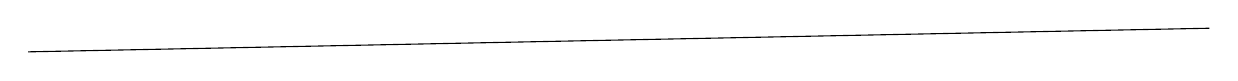
\begin{tikzpicture}\draw (0,0)--(15,0.3);\end{tikzpicture}}
$\tau_i$ réflexion strictement orthogonale
$\Longleftrightarrow(\alpha_0+2),\cdots,(\alpha_{i-1}+2)\in k^*$.
\[
(\tau_i\ \text{str. orth.}\quad\forall_{0\leq i\leq n})
\Longleftrightarrow(\alpha_i+2)\in k^*\quad\forall_{0\leq i\leq n-1}
\]
\mspage{44}

\scanpage{46}
\[
\left\{\begin{aligned}
f(s_i)&=0\qquad\varphi(s_i,s_i)=0\\
\varphi(s_i,s_j)&=-(\alpha_0+2)\cdots(\alpha_{i-1}+2)
\qquad0\leq i<j\leq n+1
\end{aligned}\right.
\]
\deleted{$f(\unsure{a_0})$}\qquad
\deleted{$f(a_0)=$}\qquad\inserted{$=c_{-2}$}
\[
\left\{\begin{aligned}
f(a_{-1})&=0,\quad
f(a_i)=(\alpha_0+2)\cdots(\alpha_{i-1}+2)=c_{i-1}
\qquad0\leq i\leq n\\
\varphi(a_i,a_j)&=0\qquad
-1\leq i\deleted{\unsure{\leq}}\inserted{<}j\leq n,
\quad\deleted{\unsure{i,j\ \text{non consécutifs}}}\\
\varphi(a_i,a_{i+1})&=-(\alpha_0+2)\cdots(\alpha_i+2)
=\deleted{\unsure{c_i}}-c_{i\deleted{\unsure{+1}}}
\qquad-1\leq i\leq n-1
\end{aligned}\right.
\]
\inserted{Attention au \unsure{chgt de notation}}
\deleted{$\unsure{2c_i}$}
\margin{$0\leq i\leq n$}
\[
\varphi(a_i,a_i)=2f(a_i)=2(\alpha_0+2)\cdots(\alpha_{i-1}+2)
\qquad0\leq i\leq n
\]
$i,j$ non consécutifs.

Matrice de $f$ p.r. à la base $(a_i)_{-1\leq i\leq n}$
\[
\deleted{\left(
\begin{array}{cccccc}
\unsure{0}&-1&&&&\\
-1&\unsure{2c_0}&\unsure{-c_0}&&&\\
&\unsure{2}&c_0&&&\\
&&c_1&&&\\
&&&&&\\
&&&&&c_{n-1}
\end{array}\right)}
\qquad
f=\left(
\begin{array}{ccccccccc}
0&-1&&&&&&&\\
-1&2&-c_0&&&&&&\\
&-c_0&2c_0&-c_1&&&&&\\
&&-c_1&2c_1&-c_2&&&&\\
&&&-c_2&2c_2&-c_3&&&\\
&&&&-c_3&2c_3&&&\\
&&&&&&\ddots&&\\
&&&&&&&2c_{n-2}&-c_{n-1}\\
&&&&&&&-c_{n-1}&2c_{n-1}
\end{array}\right)
\]
\deleted{$\det\unsure{M_f}$}
\[
\begin{aligned}
\delta(f)&=\det\left(
\begin{array}{cccccc}
-1&-c_0&0&0&&\\
0&2c_0&-c_1&0&&\\
\big|&\unsure{-}c_1&2c_1&-c_2&&\big|\\
0&0&\unsure{-}c_2&2c_2&&\big|\\
\big|&\big|&\big|&-c_3&\diagdown&2c_{n-1}\\
0&0&0&-& &
\end{array}\right)\\
&=-1\det\left(
\begin{array}{ccccc}
2c_0&-c_1&&&\\
-c_1&2c_1&-c_2&&0\\
&-c_2&\diagdown&\diagdown&\\
0&\diagdown&&&-c_{n-1}\\
&&&-c_{n-1}&2c_{n-1}
\end{array}\right)
+\underbrace{c_0\det\left(
\begin{array}{ccc}
0&-&-\\
0&&\\
\big|&-&-\\
0&-&
\end{array}\right)}_{0}
\end{aligned}
\]
\[
\det\left(
\begin{array}{cccccc}
2c_{-1}&-c_0&0&0&--&0\\
-c_0&2c_0&-c_1&&&\big|\\
0&-c_1&2c_1&&&\big|\\
\big|&&&\diagdown&&0\\
\big|&&&&\diagdown&-c_{n-1}\\
0&\text{---}&&0&-c_{n-1}&\underset{\unsure{?}}{2}c_{n-1}
\end{array}\right)
=F_{n+1}(\underbrace{c_{-1},\ldots,c_{n-1}}_{n+1\ \text{arguments}})
\]
\[
\begin{aligned}
-\delta(f)&=\unsure{\mathrel{:}}F_n(c_0,\ldots,c_{n-1})\\
&=2c_0F_{n-1}(c_1,\ldots,c_{n-1})
+c_1\det\left(
\begin{array}{cccccc}
-c_1&-c_2&\unsure{0}&0&&\\
0&2c_2&-c_3&0&&\\
\big|&-c_3&2c_3&-c_4&&\\
\big|&0&-c_4&2c_4&&\\
\big|&\big|&0&&-c_5&\\
0&0&\big|&&&\\
&&0&&\big|&c_{n-1}
\end{array}\right)\\
&=2c_0\inserted{F_{n-1}(c_1,\ldots,c_{n-1})}
\unsure{-}c_1^2F_{n-2}(c_2,\ldots,c_{n-1})
\end{aligned}
\]
\diagram{\begin{tikzcd}[ampersand replacement=\&,column sep=small]
0\arrow[r]\&1\arrow[r]\&2\arrow[r]\&3\&\cdots\arrow[r]\&n-1\arrow[r]\&0
\end{tikzcd}}
permutation \uline{circulaire $u$, $u^{-1}$}
\[
F_1(c_0)=2c_0
\]
\[
F_2(c_0,c_1)=4c_0c_1\unsure{-}c_1^2
=c_1(4c_0-c_1)
\]
\[
\begin{aligned}
F_3(c_0,c_1,c_2)&=2c_0(4c_1c_2-c_2^2)-2c_1^2c_2\\
&\deleted{=8c_0c_1c_2}\\
&=2c_2(4c_0c_1-\deleted{\unsure{2}}c_0c_2-\deleted{\unsure{2}}c_1^2)
\end{aligned}
\]
\mspage{45}

\scanpage{47}
\[
\det\bigl((c_{ij})_{1\leq i,j\leq n}\bigr)\overset{?}{=}
\qquad c_{ij}=0\quad\text{si }i\neq j,\ i,j\ \text{non consécutifs}
\]
\[
\sum_{\sigma\in\unsure{\mathfrak S}_n}
\varepsilon_\sigma\overset{\unsure{*}}{\prod_{i=1}^{n}}
\underbrace{c_{i\,\sigma(i)}}_{\text{nul, sauf si }\sigma\ \text{est tel que}}
\qquad
\overbrace{\forall i\in[1,n],\quad\sigma i\in\{i-1,i,i+1\}}^{\sigma\ \text{admissible}}
\]
Supposons $n\geq\unsure{2|3}$, alors tt cycle de $\sigma$ est de longueur $1$ ou $2$
et les cycles de long. $2$ \unsure{sont formés} d'indices consécutifs,
donc $\sigma$ est de la forme
\[
\sigma_{i_1}\sigma_{i_2}\mathbin{-}\sigma_{i_p}
\qquad1\leq i_1<i_2\mathbin{-}<i_p\leq n-1
\]
($\sigma_i$ est la transposition de $i,i+1$), où $i_1\ i_2\mathbin{-}i_p$
sont des entiers non consécutifs.
\margin{\figure{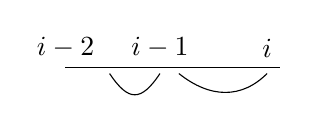
\begin{tikzpicture}[scale=.8]
\draw (0,0)--(3.4,0);
\node[above] at (0,0){$i-2$};\node[above] at (1.5,0){$i-1$};\node[above] at (3.2,0){$i$};
\draw (.7,-.1) .. controls (1,-.55) and (1.2,-.55) .. (1.5,-.1);
\draw (1.8,-.1) .. controls (2.3,-.5) and (2.8,-.5) .. (3.2,-.1);
\end{tikzpicture}}}
\[
\underbrace{1+\alpha_{\unsure{0|1}}}_{i_1}\quad
\underbrace{\deleted{\unsure{i_1+}}3+\alpha_{\unsure{0|1}}+\alpha_2}_{i_2}\quad
\underbrace{\unsure{i_1+}5+\alpha_{\unsure{0|1}}+\alpha_2+\alpha_3}_{i_3}
\mathbin{-}
\underbrace{\deleted{\unsure{i_1+}}(2\unsure{p}-1)+\alpha_{\unsure{0|1}}\mathbin{-}+\alpha_p}_{i_p}
\]
\deleted{$\displaystyle
\sum_{\substack{i_1\,i_2\,\mathbin{-}\,i_p\\
\text{\unsure{entiers} str. cr.}\\\text{distants}}}$}
\[
\deleted{1\leq i_1\qquad1+\alpha_1\mathbin{-}+\alpha_{p-1}\leq}
\]
\[
\alpha_i\in\mathbb N\qquad
\alpha_0\mathbin{-}+\alpha_{p-1}\leq n-2p
\]
\[
\begin{aligned}
&\sum_{1\leq p\leq[\frac n2]}(-1)^p
\sum_{\substack{(\alpha_{\unsure{0|1}},\ldots,\alpha_{\unsure{p-1|p}})\in\mathbb N^p\\
\sum\alpha_i=n-2p}}
\deleted{\unsure{\prod_i}}
\prod_{\substack{1\leq i\leq n\\
\text{non de la forme}\\
\left\{\begin{smallmatrix}(2r-1)+(\alpha_{\unsure{0|1}}\mathbin{-}+\alpha_r)\\
2r+(\alpha_{\unsure{0|1}}\mathbin{-}+\alpha_r)\end{smallmatrix}\right.\\
1\leq r\leq p}}
c_{ii}\\
&\hspace{3em}\prod_{1\leq r\leq p}
\left(
c_{2r-1+(\alpha_1+\cdots+\alpha_r),\,2r+(\alpha_1+\cdots+\alpha_r)}
c_{2r+(\alpha_1+\cdots+\alpha_r),\,2r-1+(\alpha_1\mathbin{-}+\alpha_r)}
\right)
\end{aligned}
\]
Supposons matrice \uline{symétrique}, et
$c_{i\,i+1}=-c_{i+1}\qquad c_{ii}=2c_i$.

On trouve
\[
\det\bigl((c_{ij})\bigr)_{1\leq i,j\leq n}
=\sum_{1\leq p\leq[\frac n2]}(-1)^p
2^{\inserted{\text{\figure{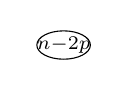
\begin{tikzpicture}[baseline=-.5ex]
\draw (0,0) ellipse (.34 and .18);\node at (0,0){$\scriptstyle n-2p$};
\end{tikzpicture}}}}}
\sum_{\substack{\alpha_*\in\mathbb N^p\\
\alpha_1\mathbin{-}+\alpha_p\leq n-2p}}
\prod_i c_i
\prod_{1\leq r\leq p}
(c_{2r+\alpha_1\mathbin{-}+\alpha_r})^2
\]
\figure{\begin{tikzpicture}[x=.65cm,y=.65cm]
\fill (0,0) circle (.035);\node[below] at (0,-.08){$c_1$};
\draw (.4,0)--(1.2,0);\draw (.4,-.08)--(.4,.08);\draw (1.2,-.08)--(1.2,.08);
\node[below] at (.65,-.08){$c_2$};
\draw (1.4,0)--(2.35,0);\draw (1.4,-.08)--(1.4,.08);\draw (2.35,-.08)--(2.35,.08);
\node[below] at (1.4,-.08){$c_3$};
\fill (2.5,0) circle (.055);\draw (2.5,0)--(3.2,0);\fill (3,0) circle (.07);
\draw (3.3,-.08)--(3.3,.08);\draw (3.3,0)--(4.2,0);\draw (4.2,-.08)--(4.2,.08);
\fill (4.5,0) circle (.035);
\draw (4.8,-.08)--(4.8,.08);\draw (4.8,0)--(6,0);\draw (6,-.08)--(6,.08);
\node at (6.65,0){$\cdots$};
\draw (7.3,-.08)--(7.3,.08);\draw (7.3,0)--(8.8,0);\fill (8.8,0) circle (.035);
\node at (9.4,0){$\cdots$};\node[below] at (9.8,-.08){$c_n$};
\fill (-.4,-.65) circle (.025);\node at (-2,-1.65){$c$};
\end{tikzpicture}}
\mspage{46}

\scanpage{48}
\[
\langle a_i,a'_j\rangle=
\begin{cases}
0&\text{si }i\neq j,\ i\text{ et }j\text{ non consécutifs}\\
1&\text{si }\deleted{\unsure{i,j\ \text{consécutifs}}}\quad i=j-1\\
\deleted{\unsure{2}}\lambda_j-1&\text{si }\deleted{\unsure{j=i}}\quad i=j\\
-\lambda_j+1+\alpha_j&\deleted{\unsure{\text{si }j=i-1}}\quad i=j+1
\end{cases}
\]
\[
a_i=s_{i+1}-s_i
\]
\[
a'_j=s_j^*+\lambda_js_{j+1}^*+(1+\alpha_j)
(s_{j+2}^*\mathbin{-}+\unsure{s_{n-1}^*|s_{n+1}^*})
\qquad0\leq j\leq n
\]
\[
a'_n=
\]
\[
\left\{\begin{aligned}
a'_j&=a_{j-1}^*
+\underbrace{(\lambda_j-1)}_{-2\ \text{si }\lambda_j=-1}a_j^*
+\underbrace{(1-\lambda_j+\alpha_j)}_{\beta_j=2+\alpha_j\ \text{si }\lambda_j=-1}
a_{j+1}^*
\qquad0\leq j\leq n-1\\
a'_n&=a_{n-1}^*+(\lambda_n-1)a_n^*\deleted{\unsure{+}}\\
\Pi&=a_{-1}^*\\
s_j&=a_{-1}+\cdots+a_{j-1}\qquad0\leq j\leq n+1
\end{aligned}\right.
\]
\margin{\[
\deleted{\boxed{\begin{aligned}
\Psi(a_{-1})&=-a_0^*\\
\Psi(a_n)&=-c_{n-2}a_{n-1}^*+2c_{n-1}a_n^*
\end{aligned}}}
\]}
\[
f(a_i)\deleted{\unsure{\varphi}}a'_i+\Psi(a_i)=0
\]
\[
f\left(\sum_{-1}^{n}\zeta_i a_i\right)
=\sum_{i=0}^{n}c_{i-1}\zeta_i^2
-\sum_{-1\leq i\deleted{\unsure{j}}\leq n-1}c_i\zeta_i\zeta_{i+1}
\]
\[
\deleted{\Psi(a_i)=-c_{i-1}a_{i-1}^*+2c_{i-1}a_i^*-c_i a_{i+1}^*}
\qquad0\leq i\leq n-1
\]
\figure{\begin{tikzpicture}
\draw (4,4) .. controls (3,2.8) and (1,3.3) .. (.2,1.5)
.. controls (-.4,.5) and (.3,0) .. (.8,0);
\end{tikzpicture}}
\margin{Cas où pour \deleted{\unsure{\text{tous les indices}}}
\[
\begin{gathered}
c_{-1}=1,\quad c_0=(\alpha_0+2),\ldots,\quad
c_i=(2+\alpha_0)\mathbin{-}(2+\alpha_i)
\quad0\leq i\leq n-1\\
\unsure{0\leq i\leq n}\qquad c_n=c_{n+1}=0
\end{gathered}
\]}
Coordonnées projectives de $c$, orth. aux $a'_i$

(en fait $\lambda_i=-1$ pour $0\leq i\leq n$)
\[
c'=\sum_{-1}^{n}\zeta_i a_i\qquad(\zeta_n=1)
\]
\[
\zeta_{n-1}-2\zeta_n=0\qquad
\deleted{\unsure{\zeta_{n-1}=2}}
\boxed{\zeta_n=1,\ \zeta_{n-1}=2}
\]
\[
\zeta_{n-2}-2\zeta_{n-1}+(\alpha_{n-1}+2)\zeta_n=0
\qquad\boxed{\zeta_{n-2}=-(\alpha_{n-1}-2)}
\]
\[
\zeta_{n-3}
+\underbrace{-2\zeta_{n-2}+(\alpha_{n-2}+2)\zeta_{n-1}}_{
\begin{smallmatrix}2(\alpha_{n-1}-2)+(\alpha_{n-2}+2)2\\
=2(\alpha_{n-1}+\alpha_{n-2})\end{smallmatrix}}
=0
\qquad\boxed{\zeta_{n-3}=-2(\alpha_{n-1}+\alpha_{n-2})}
\]
\[
\zeta_{n-4}\unsure{-} \underbrace{
2\zeta_{n-3}+(\alpha_{n-3}+2)\zeta_{n-2}}_{
4(\alpha_{n-1}+\alpha_{n-2})\unsure{-}(\alpha_{n-3}+2)
\underbrace{(\alpha_{n-1}-2)}}
=0
\]
\margin{\[
\boxed{\begin{aligned}
\zeta_{n-4}&=\deleted{\unsure{\alpha_{n-1}(\alpha_{n-3}+2)+4\alpha_{n-2}+4+}}\\
&-4-2(\alpha_{n-1}+2\alpha_{n-2}+\alpha_{n-3})
+\alpha_{n-1}\alpha_{n-3}
\end{aligned}}
\]}
\[
2\uline{\alpha_{n-1}}+4\uline{\alpha_{n-2}}+\uline{4}
-\uline{\alpha_{n-1}\alpha_{n-3}}+2\uline{\alpha_{n-3}}
\]
\[
\zeta_{n-5}=\mathbin{---}
\]
\[
\Pi=a_{-1}^*
\]
\[
\Pi(c')=\rho(\underbrace{\alpha_0,\ldots,\alpha_{n-1}}_A)
=\rho=\zeta_{-1}
\qquad\rho\in\mathbb Z[A_0,\ldots,A_{n-1}]
\]
\[
c=\frac{c'}{\rho}
\]
\[
f(c')=\underbrace{\sigma(\alpha_0,\mathbin{-}\alpha_{n-1})}_{
\sigma\in\mathbb Z[A_0,\mathbin{-}A_{n-1}]}
=\sigma
\]
\[
f(c)=\sigma/\rho^2\qquad
2\sigma=-\zeta_0\zeta_{-1}=-\rho\zeta_0
\]
\[
2f(c')=\langle c',\Psi(c')\rangle\overset{?}{=}
\]
\[
\deleted{\Psi(c')=\inserted{\lambda\Pi=}\lambda a_{-1}^*
\qquad\lambda=\langle a_{-1},\Psi(c')\rangle
=\varphi(a_{-1},c')}
\]
\[
\begin{aligned}
\langle a_i,\Psi(c')\rangle
&=\varphi(a_i,c')=\langle c',\underbrace{\Psi(a_i)}_{
-f(a_i)a'_i\ /\ \text{si }0\leq i\leq n}\rangle
=\deleted{\unsure{\lambda\zeta_i}}\\
&=-f(a_i)\langle c',a'_i\rangle
=0\quad\deleted{\unsure{\text{si }0\leq i\leq n}}\\
\langle a_{\deleted{\unsure{0}}\inserted{-1}},\Psi(c')\rangle
&=\langle c',\underbrace{\Psi(a_{-1})}_{-a_0^*}\rangle
=-\deleted{\unsure{\zeta_{-1}}}\zeta_0=
\end{aligned}
\]
\[
\Psi(c')=-\zeta_0a_{-1}^*
\]
\[
2f(c')=\langle c',-\zeta_0a_{-1}^*\rangle=-\zeta_0\zeta_{-1}
\]
\mspage{47}

\scanpage{49}
\inserted{$\Delta_{n+2}(0,1,c_0,\ldots,c_{n-1})$}
\[
\deleted{\unsure{\Delta}}
\Delta_n(\underbrace{c_0,\ldots,c_{n-1}}_{n\ \text{arg.}})
=\unsure{-}\det\left(
\begin{array}{ccccccccc}
0&-1&0&0&0&0&0&\cdots&0\\
-1&2&-c_0&0&0&0&0&\cdots&0\\
0&-c_0&2c_0&-c_1&0&0&0&\cdots&\vdots\\
0&0&-c_1&2c_1&-c_2&-c_3&0&&\vdots\\
0&0&0&&&&&&0\\
\vdots&\vdots&\vdots&&&&&&-c_{n-1}\\
0&0&0&--&0&&&-c_{n-1}&2c_{n-1}
\end{array}\right)
\quad(\text{ordre }n+2)
\]
\[
=\det\left(
\begin{array}{ccccccc}
2c_0&-c_1&0&0&0&\text{---}&0\\
-c_1&2c_1&-c_2&0&0&&\\
0&-c_2&2c_2&-c_3&0&--&\big|\\
0&0&-c_3&2c_3&-c_4&&0\\
--&--&--&--&\text{---}&--&-c_{n-1}\\
0&0&0&0&\cdots&-c_{n-1}&2c_{n-1}
\end{array}\right)
\quad\text{ordre }n
\]
\[
\boxed{\Delta_n(c_0,\ldots,c_{n-1})
=2c_0\Delta_{n-1}(c_1,\ldots,c_{n-1})
\unsure{-}c_1^2\Delta_{\unsure{n-1|n-2}}(c_2,\ldots,c_{n-1})}
\]
\[
\Delta'_n(c_0,\ldots,c_{n-1})=
\begin{cases}
\Delta_n(c_0,\ldots,c_{n-1})&\text{si }n\ \deleted{\unsure{\text{im}}}\text{pair}\\
\frac12\Delta_n(c_0,\ldots,c_{n-1})&\text{si }n\text{ impair}
\end{cases}
\]
Posons
\[
\left.\begin{aligned}
c_0&=\beta_0,\ \unsure{c}\\
c_1&=\beta_0\beta_1\\
&\mathbin{--}\\
c_{n-1}&=\beta_0\beta_1\mathbin{-}\beta_{n-1}
\end{aligned}\right\}
\quad n\ \text{indéterminées }\beta_i
\]
\[
\delta_n(\beta_0,\ldots,\beta_{n-1})
=\Delta_n(\beta_0,\beta_0\beta_1,\ldots,\beta_0\beta_1\mathbin{-}\beta_{n-1})
\]
\[
\delta'_n(\beta_0,\ldots,\beta_{n-1})=\Delta'_n(\ldots)
=\begin{cases}
\delta_n(\beta_0,\mathbin{-}\beta_{n-1})&n\text{ pair}\\
\frac12\delta_n(\beta_0,\mathbin{-}\beta_{n-1})&n\text{ impair}
\end{cases}
\]
\[
\Delta_n,\Delta'_n,\deleted{\unsure{\widetilde\Delta_n}}
\inserted{\widetilde\Delta'_n}\in\mathbb Z[C_0,\ldots,C_{n-1}]
\]
\[
\delta_n,\delta'_n,\widetilde\delta'_n\in\mathbb Z[B_0,\ldots,B_{n-1})
\]
\margin{\[
\begin{aligned}
\Delta'_n[C_0,\mathbin{-},C_{n-1}]
&=C_{n-1}\widetilde\Delta'_{n-1}(C_0,\mathbin{-},C_{n-2})\\
\delta'_n[B_0,\mathbin{-},B_{n-1}]
&=B_{n-1}\widetilde\delta'_n(B_0,\ldots,B_{n-2})
\end{aligned}
\]}
\[
\Delta_1(c_0)=2c_0,\quad\Delta'_1(c_0)=c_0
\qquad\widetilde\Delta'_1(c_0)=1
\]
\[
\Delta_2(c_0,c_1)=4c_0c_1-c_1^2=c_1(4c_0-c_1)
\qquad\widetilde\Delta'_2(c_0,c_1)=4c_0-c_1)
\]
\[
\Delta_3(c_0,c_1,c_2)=2c_2(4c_0c_1-c_0c_2-c_1^2),\quad
\Delta'_3=\deleted{\unsure{2}}c_2(4c_0c_1-c_0c_2-c_1^2),
\]
\[
\mathbin{---}\qquad
\widetilde\Delta'_3(c_0,c_1,c_2)=4c_0c_1-c_0c_2-c_1^2
\]
\[
\Delta_n(C_0,\mathbin{-},C_{n-1})
=\sum_{0\leq p\leq[\frac n2]}(-1)^p2^{n-2p}
\sum_{\substack{\text{suites de }p\\
\deleted{\unsure{\text{intervalles}}}\\
\text{él. de }\unsure{\mathcal P}_2([0,n-1])\\
\text{disjoints}\\
J_1\mathbin{-}J_p,\ \deleted{\unsure{J_i=\{j_i,j_i+1\}}}}}
\prod_{i\in J'}C_i\prod_{j\in J''}C_j^2
\]
\[
J=\bigcup_{1\leq i\leq p}J_i,\qquad
J'=[0,n-1]\setminus J
\]
$J''=$ ens des derniers él'mts des $J_i$
\[
(J''\in\unsure{\mathcal P}_p([0,n-1]))
\]
\margin{\unsure{chgt} notation}
\margin{non, grâce au \unsure{régime} des paires}
\figure{\begin{tikzpicture}
\draw[->] (1.5,1)..controls(1,.5)and(.4,.4)..(0,.2);
\draw (2,1)--(2,.15);
\end{tikzpicture}}
\margin{\uline{NB} Il n'y a pas de cancellation de termes.}

\deleted{$\unsure{\Delta_n(C_0,\ldots,C_{n-1})=}$}
Le monôme $M=\prod_{i\in J'}C_i\prod_{j\in J''}C_j^2$
s'écrit aussi
\[
\deleted{\unsure{\delta_n(c_1,\ldots,c_n)=\beta_0}}
\]
\[
B_0^n B_1^{n-1+\varepsilon_2}
B_{\unsure{3|2}}^{n-2+\varepsilon_3}\mathbin{-}B_{n-1}^{\varepsilon_n}
\]
\[
\varepsilon_k\in\{0,1\}\qquad2\leq k\leq n
\]
\[
\varepsilon_k=1\ \text{sss}\ k\in J'''
\]
(il y en \unsure{a} $p$ tels $k$)
\[
M=\prod_{1\leq i\leq n}C'_i\qquad
C'_i=\begin{cases}
C_i&\text{si }i\in J'\\
C_j&\text{si }j\in J''\\
C_{j+1}&\text{si }j\in\deleted{\unsure{J''}}\inserted{J'''}
\end{cases}
\]
\figure{\begin{tikzpicture}[x=1cm,y=.6cm]
\draw (0,0)--(5,0);
\fill (.15,0) circle (.025);\node[below] at (.15,0){$1$};
\fill (2.3,.08) circle (.025);\node[below] at (2.3,0){$k$};
\fill (4.8,.1) circle (.025);\node[above] at (4.8,.1){$n$};
\end{tikzpicture}}
\[
\delta_n(B_0,\ldots,B_n)
=B_0^nB_1^{n-1}\cdots B_{n-1}^{1}
\underbrace{\unsure{L_n|L_{n-1}}(B_1,\mathbin{-},B_{n-1})}_{
\text{polynôme }\deleted{\text{de degré}}\ \leq[\frac n2]}
\]
\margin{\figure{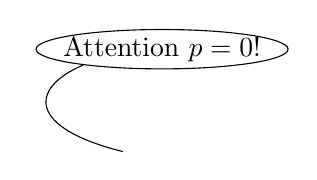
\begin{tikzpicture}
\draw (0,0) ellipse (1.6 and .25);
\node at (0,0){Attention $p=0$!};
\draw (-1,-.2)..controls(-1.7,-.5)and(-1.7,-1)..(-.5,-1.3);
\end{tikzpicture}}}
\deleted{\unsure{Attention!}}
$C'_i$ contient un facteur \uline{$B_k$}
\deleted{\unsure{(et une puissance)}}
(à la puiss. $1$ exactement) sss
\deleted{\unsure{\text{au moins}}}
$i\geq k$, \uline{ou} $i=k-1$ \uline{et}
$i\in J'''$ i.e. $k\in J''$.
\[
\begin{aligned}
\unsure{L_n|L_{n-1}}(B_1,\mathbin{-},B_{n-1})
&=\sum_{0\leq p\leq[\frac n2]}(-1)^p2^{n-2p}
\sum_{\substack{\deleted{\unsure{\text{suite de }p\text{ intervalles}}}\\
\deleted{\unsure{J''}}\ J\in\unsure{\mathcal P}_p([1,n-1])\\
J\ \text{ne contient pas }2\\\text{entiers consécutifs}}}
B_J\\
&=2^n\unsure{-}2^{n-2}\sum_{\unsure{0\leq i\leq n-1}}B_i
+2^{n-4}\sum_{\substack{1\leq i<j\leq n-1\\j\neq i+1}}B_iB_j\\
&\quad-2^{n-6}\sum_{\substack{1\leq i<j<k\leq n\\\unsure{\vdots\quad\vdots}}}
B_iB_jB_k+\cdots
\end{aligned}
\]
\margin{Attention, $n-1$ et non $n$!}
\mspage{48}

\scanpage{50}
\[
\deleted{\Pi_p(B_1,\mathbin{-},B_n)=\sum_{J\in\unsure{\mathcal P}_p[1,n]}}
\qquad B_i=B'_i+4
\]
\deleted{$\unsure{\Sigma}$}
\[
B'_1B'_2=B'_2B'_3=\mathbin{--}=B'_nB'_{n-1}=0
\]
\[
(2-\tfrac{B_1}{2})(2-\tfrac{B_2}{2})\cdots(2-\tfrac{B_n}{2})
=\frac{(-1)^n}{2^n}.
\]
\[
L_1=2\qquad L'_1=1
\]
\[
L_2=4-B_1\deleted{\unsure{+B_2}}
=\deleted{\unsure{4-(\alpha_0+\alpha_1)-\alpha_0+}}
2-\alpha_0=-(\alpha_0-2)
\]
\[
L_3=8-2(B_1+B_2\deleted{\unsure{+B_3}})
=-2[\alpha_1+\alpha_2+\deleted{\unsure{\alpha_0+\alpha_1}}]
\]
\[
L_4=\underbrace{16-4(B_1+B_2+B_3+\deleted{\unsure{B_4}})
+\left(\sum_{1\leq i\leq j\leq3}B_iB_j\right)}
-(B_1B_2+B_2B_3+B_3B_4)
\]
\[
\deleted{(2-\tfrac{B_1}{2})(2-\tfrac{B_2}{2})}
\]
\[
\begin{aligned}
&-4(\alpha_1+\alpha_2+\alpha_3+\deleted{\unsure{\alpha_4}})-8\\
&\quad+\bigl[
\deleted{(\alpha_0+2)(\alpha_1+2)}
+(\alpha_0+2)(\alpha_2+2)
+\deleted{\unsure{(\alpha_1+2)(\alpha_3+2)}}\\
&\hspace{8em}+\deleted{\unsure{(\alpha_2+2)(\alpha_3+2)}}\bigr]
\end{aligned}
\]
\[
\deleted{\begin{aligned}
=&-4-4(\alpha_0+\alpha_1+\alpha_2\deleted{\unsure{+\alpha_3}})
+2(\alpha_0+\alpha_1+\alpha_2+\alpha_3+\alpha_2+\alpha_3)\\
&+\alpha_0\alpha_2+\alpha_0\alpha_3
\end{aligned}}
+\alpha_1\alpha_3
\]
\[
\deleted{\unsure{2\alpha_0+2\alpha_1+2\alpha_2+2\alpha_3}}
\]
\[
\begin{aligned}
&=-4-2(\alpha_1+\inserted{2\alpha_2+}\alpha_3)
+(\alpha_1\alpha_3\deleted{\unsure{+\alpha_0\alpha_3+\alpha_2\alpha_3}})\\
&=(\alpha_1-2)(\alpha_3-2)\unsure{-}4(\alpha_2+2)
\end{aligned}
\]
\figure{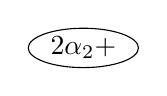
\begin{tikzpicture}
\draw (0,0) ellipse (.7 and .25);\node at (0,0){$2\alpha_2+$};
\end{tikzpicture}}
\uline{NB}\quad
$L_{n-1}(B_1,\mathbin{-},B_{n-1})
=L_{n-1}(B_{n-1},\ldots,B_1)$
\figure{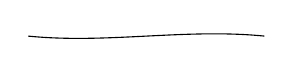
\begin{tikzpicture}\draw (0,0)..controls(1,-.1)and(2,.1)..(3,0);\end{tikzpicture}}
\[
\begin{aligned}
&\det\left(
\begin{array}{cccccc}
2\deleted{\unsure{C_{-1}}}&-C_0&0&&&\\
-C_0&2C_0&-C_1&0&&\\
0&-C_1&2C_1&&&0\\
0&0&-C_2&\ddots&C_{n-2}&-C_{n-1}\\
&--&&0&-C_{n-1}&2C_{n-1}
\end{array}\right)\\
&=\Delta_{n+1}(\underbrace{1,C_0,\mathbin{-},C_{n-1}}_{n+1\ \text{arg.}})
=2\Delta_n(C_0,\mathbin{-},C_{n-1})
-C_0^2\Delta_{n-1}(C_1,\mathbin{-},C_{n-1})
\end{aligned}
\]
\inserted{\deleted{\unsure{n+1}}\quad ordre $n+1$}
\[
=\delta_{n+1}(1,B_0,\ldots,B_{n-1})
=B_0^nB_1^{n-1}\mathbin{-}B_{n-1}
L_{n+1}(\deleted{\unsure{1}}B_0,\mathbin{-},B_{n-1})
\]
\[
\deleted{L_2(1,B_0)=4-}
\]
\[
\deleted{\unsure{\tfrac12\delta_{n+1}(1,B_0,\ldots,B_{n-1})}}
\qquad
\deleted{L_3(\unsure{1},B_0,}
\]
\[
\delta_2(1,B_0)\deleted{\unsure{B_1}}
=B_0L_2(1,B_0)=B_0(4-B_0)
=-(\alpha_0+2)(\alpha_0-2)=4-\alpha_0^2
\]
\[
\delta'_3(1,B_0,B_1)
=B_0^2B_1L'_3(\deleted{\unsure{1}}B_0,B_1)
=\deleted{\unsure{B_0^2B_1}}\deleted{\unsure{2}}
-B_0^2B_1(\alpha_0+\alpha_1)
\]
\[
\delta_4(1,B_0,B_1,B_2)
=B_0^3B_1^2B_2
\underbrace{L_4(B_0,B_1,B_2)}_{(\alpha_0-2)(\alpha_2-2)-4(\alpha_1+2)}
\]
\margin{\[
\deleted{\begin{aligned}
\det\begin{pmatrix}2C_0&-C_1\\-C_1&2C_1\end{pmatrix}
&=4C_0C_1-C_1^2\\
&=C_1(4C_0-C_1)\\
&=B_0^2B_1(4-B_1)
\end{aligned}}
\]}
\mspage{49}

\scanpage{51}
\[
\left\{\begin{aligned}
\delta_n(B_0,\ldots,B_{n-1})
&=B_0^nB_1^{n-1}\mathbin{-}B_{n-1}L_n(B_1,\mathbin{-},B_{n-1})\\
\delta_{n+1}(1,B_0,\ldots,B_{n-1})
&=B_0^nB_1^{n-1}\mathbin{-}B_{n-1}L_{n+1}(B_0,B_1,\ldots,B_{n-1})
\end{aligned}\right.
\]
\[
\left\{\begin{aligned}
\delta'_n(B_0,\mathbin{-},B_{n-1})
&=B_0^nB_1^{n-1}B_{n-1}L'_n(B_1,\mathbin{-},B_{n-1})\\
\delta'_{n+1}(1,B_0,\ldots,B_{n-1})
&=B_0^nB_1^{n-1}\mathbin{-}B_{n-1}L'_{n+1}(B_0,B_1,\mathbin{-},B_{n-1})
\end{aligned}\right.
\]
\deleted{$n$ pair
$\left\{\begin{aligned}
L_n(B_1,\mathbin{-},B_{n-1})&\equiv B_1B_3\mathbin{-}B_{n-1}\\
\delta_n(
\end{aligned}\right.$}
\figure{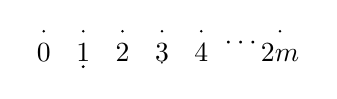
\begin{tikzpicture}[x=.5cm,y=.5cm]
\foreach \x/\s in {0/0,1/1,2/2,3/3,4/4,6/{2m}}
{\fill (\x,0) circle (.035);\node[below] at (\x,-.08){$\s$};}
\fill (1,-.9) circle (.04);\fill (3,-.8) circle (.025);
\node at (5,-.3){$\cdots$};
\end{tikzpicture}}
\[
L_{2m}(B_1,\mathbin{-},B_{2m-1})
\equiv B_1B_3\cdots B_{2m-1}
\qquad\uuline{\text{mod }2}
\]
\[
\begin{aligned}
L'_{2m+1}(B_1,\mathbin{-},B_{2m})
&\equiv(B_2B_4\mathbin{-}B_{2m}
+B_1B_3\unsure{B_5B_7}\cdots B_{2m-1})\\
&\quad+\sum_{1\leq i\leq m-1}
(B_1\mathbin{-}B_{2i-1})(B_{2i+2}\mathbin{-}B_{2m})
\end{aligned}
\]
\[
\left\{\begin{aligned}
\delta_{2m}^{\unsure{'|*}}(B_0,\mathbin{-},B_{2m-1})
&\equiv
\deleted{\unsure{(B_0^{2m}B_1^{2m-1}\mathbin{-})}}
\underbrace{(B_0B_1)^{2m}(B_2B_3)^{2(m-1)}
\mathbin{-}(B_{2m-2}B_{2m-1})}_{
[(B_0B_1)^m(B_2B_3)^{m-1}\mathbin{-}(B_{2m-2}B_{2m-1})]^2}\\
&\quad\deleted{\unsure{\delta_{2m}\cdots}}\\
\delta'_{2m+1}(1,B_0,\mathbin{-},B_{2m-1})
&\equiv B_0^{2m}B_1^{2m-1}\mathbin{-}B_{2m-1}
\bigl[B_0B_2\mathbin{-}B_{2m-2}+B_1B_3\mathbin{-}B_{2m-1}\\
&\hspace{8em}+\sum_{1\leq i\leq m-1}
(B_0\mathbin{-}B_{2i-2})(B_{2i+1}\mathbin{-}B_{2m-1})\bigr]
\end{aligned}\right.
\]
\[
\left\{\begin{aligned}
\delta'_{2m+1}(B_0,\mathbin{-},B_{2m})
&\equiv B_0^{2m+1}B_1^{2m}\mathbin{-}B_{2m}
\bigl(B_2B_4\mathbin{-}B_{2m}+B_1B_3\mathbin{-}B_{2m-1}\\
&\hspace{8em}+\sum_{1\leq i\leq m-1}
(B_1\mathbin{-}B_{2i-1})(B_{2i+2}\mathbin{-}B_{2m})\bigr)\\
\delta_{2m+2}(1,B_0,\mathbin{-},B_{2m})
&\equiv\deleted{\unsure{(B_0^{2m+1}B_1^{m+1})}}
[B_0^{m+1}(B_1B_2)^m\cdots(B_{2m-1},B_{2m})]^2
\end{aligned}\right.
\]
\mspage{50}

\scanpage{52}
\[
\Delta_n(\unsure{C_0},\mathbin{-},\unsure{C_{n-1}|C_n})
=2C_0\Delta_{n-1}(C_1,\mathbin{-},C_{n-1})
-C_1^2\Delta_{\unsure{n-1|n-2}}(C_2,\mathbin{-},C_{n-1})
\]
\[
\begin{aligned}
\delta_n(B_0,\mathbin{-},B_{n-1})
&=2B_0\delta_{n-1}(B_0B_1,B_2,\mathbin{-},B_{n-1})
-(B_0B_1)^2\delta_{n-2}(B_0B_1B_2,B_3,\ldots,B_{n-1})\\
&=2B_0^{\unsure{n|1}}(B_0B_1)^{n-1}B_2^{n-2}B_3^{n-3}
\mathbin{-}B_{n-1}L_{n-1}(\deleted{\unsure{B_0}}B_2,B_3,\mathbin{-},B_{n-1})\\
&\quad-B_0^2B_1^2(B_0B_1B_2)^{n-2}B_3^{n-3}
\mathbin{-}B_{n-1}L_{n-2}(B_3,\ldots,B_{n-1})\\
&=B_0^nB_1^{n-1}\mathbin{-}B_{n-1}
[2L_{n-1}(B_2,\mathbin{-},B_{n-1})-B_1L_{n-2}(B_3,\ldots,B_{n-1})]
\end{aligned}
\]
\margin{$B_0^n\mathbin{-}B_{n-1}L_n(B_1,\ldots,B_{n-1})$}
\[
\boxed{L_n(B_1,\ldots,B_{n-1})
=2L_{n-1}(B_2,\ldots,B_{n-1})-B_1L_{n-2}(B_3,\ldots,B_{n-1})}
\]
\[
\left\{\begin{aligned}
L_{2m}^{\deleted{\unsure{'}}}(B_1,\mathbin{-},B_{2m-1})
&=4L'_{2m-1}(B_2,\mathbin{-},B_{2m-1})
-B_1L_{2m-2}(B_3,\mathbin{-},B_{2m-1})\\
L'_{2m+1}(B_1,\mathbin{-},B_{2m})
&=\deleted{\unsure{2}}L_{2m}(B_2,\mathbin{-},B_{2m})
-B_1L'_{2m-1}(B_3,\ldots,B_{2m})
\end{aligned}\right.
\]
Calcul de $\unsure{\widetilde o|\widetilde c}$ défini par
\[
\unsure{\parallel|=}\quad\zeta_{-1}a_{-1}+\zeta_0a_0\mathbin{-}+\zeta_na_n
\qquad
\left\{\begin{aligned}
\zeta_n&=1\\
\langle\unsure{\widetilde o|\widetilde c},a'_{\unsure{0|i}}\rangle&=0
\qquad0\leq i\leq n
\end{aligned}\right.
\]
i.e.
\[
\left\{\begin{aligned}
\zeta_n&=1\\
\zeta_{n-1}&=2\\
\bigl\{\ \zeta_{i-1}-2\zeta_i+\beta_i\zeta_{i+1}&=0
\qquad0\leq i\leq n-1\\
\zeta_{i-1}&=2\zeta_i\unsure{\div|-}\beta_i(\zeta_{i+1})
\end{aligned}\right.
\]
\[
\zeta_n=1,\quad\zeta_{n-1}=2,\quad\zeta_{n-2}=4-\beta_{n-1},\quad
\zeta_{n-3}=2(4-\beta_{\unsure{n-2|n-1}})
-2\beta_{n-2}\unsure{\cdot2}
=8-2(\beta_{n-1}+\beta_{n-2})
\]
\[
\boxed{\zeta_{n-i}=L_i(\underbrace{\beta_{n-1},\ldots,\beta_{n-i+1}}_{i-1\ \text{arguments}})}
\qquad1\leq i\leq n+1
\]
en particulier
\[
\rho=\unsure{\bar\zeta_{-1}|\widetilde\zeta_{-1}}
=\Pi(\unsure{\widetilde o|\widetilde c})
=L_{n+1}(\beta_{n-1},\ldots,\beta_0)
=L_{n+1}(\beta_0,\mathbin{-},\beta_{n-1})
\]
\[
\begin{aligned}
\sigma=\zeta_0
&=\langle\unsure{\widetilde o|\widetilde c},a_0^*\rangle
=\bigl[-\langle\unsure{\widetilde o|\widetilde c},\Psi(\underbrace{a_{-1}}_{s_0})\rangle
=-\varphi(\unsure{\widetilde o|\widetilde c},a_{-1})
\deleted{\unsure{\langle a_{-1},\Psi(a_{-1})\rangle}}
\inserted{=-\langle a_{-1},\Psi(\unsure{\widetilde o|\widetilde c})\rangle}\bigr]\\
&=L_n(\beta_{n-1},\ldots,\beta_1)\\
&\unsure{=}L_n(\beta_1,\mathbin{-},\beta_{n-1})
\end{aligned}
\]
\mspage{51}

\scanpage{53}
\[
\begin{aligned}
\rho&=L_{n+1}(\beta_0,\ldots,\beta_{n-1})
&\rho'&=L'_{n+1}(\beta_0,\mathbin{-}\beta_{n-1})\\
\sigma&=L_n(\beta_0,\ldots,\beta_{n-1})
&\sigma'&=L'_n(\beta_1,\mathbin{-},\beta_{n-1})
\end{aligned}
\]
\[
\left\{\begin{aligned}
\delta_{\mathcal E}&=(\overbrace{\beta_0^n\beta_1^{n-1}\mathbin{-}\beta_{n-1}}^B)\sigma\\
\delta_V&=(\underbrace{\beta_0^n\beta_1^{n-1}\mathbin{-}\beta_{n-1}}_B)\rho
\end{aligned}\right.
\qquad
\left\{\begin{aligned}
\delta'_{\mathcal E}&=(\overbrace{\beta_0^n\beta_1^{n-1}\mathbin{-}\beta_{n-1}}^B)\sigma'\\
\delta'_V&=(\underbrace{\beta_0^n\beta_1^{n-1}\mathbin{-}\beta_{n-1}}_B)\rho'
\end{aligned}\right.
\]
\margin{\[
\widetilde o=\rho a_{-1}+\sigma a_0+\zeta_1a_1\mathbin{-}+\zeta_na_n
\qquad(\zeta_n=1,\zeta_{n-1}=2\ldots)
\]}
\[
\rho=\zeta_{-1}=\Pi(\widetilde o)=\langle\widetilde o,a_{-1}^*\rangle
\]
\[
\sigma=\zeta_0=\langle\widetilde o,a_0^*\rangle
=-\varphi(\underbrace{s_0,\widetilde o}_{\unsure{\text{si }0\leq n}})\unsure{\big)}
\]
\[
\left\{\begin{aligned}
o&=\widetilde o/\rho\\
\Psi(\widetilde o)&=-\sigma a_{-1}^*=-\sigma\Pi
\end{aligned}\right.
\]
\margin{\[
o'=2o=
\left\{\begin{aligned}
&\deleted{\unsure{2}}\widetilde o/\rho'&&n\text{ pair}\\
&\deleted{\unsure{\widetilde o/\rho'}}
2\widetilde o/\rho&&n\text{ impair}\\
&\text{''}\quad2\widetilde o/\rho'
\end{aligned}\right.
\]}
\[
\begin{aligned}
f(\widetilde o)
&=\bigl[\tfrac12\langle\widetilde o,\Psi(\widetilde o)\rangle
=-\tfrac12\langle\widetilde o,\sigma\Pi\rangle
=-\tfrac12\sigma\Pi(\widetilde o)
=-\tfrac12\sigma\rho\bigr]\\
&=-\sigma'\rho'
\end{aligned}
\]
\[
\left[
\underbrace{f(o')}_{\unsure{\text{en ver}}}
=f(\widetilde o/\rho')
=\deleted{\unsure{4}}-\frac{\sigma'\rho'}{\rho'^2}
\deleted{\unsure{4}}
=-\frac{\sigma'}{\rho'}
\right]
\]
$f_{\mathcal E}$ lisse
$\Longleftrightarrow$ les $\beta_i$ $(0\leq i\leq n-1)$ inversibles,
et $\sigma'$ inv.
\[
\underset{\substack{\text{si }2\text{ inv.}\\\text{ou }n\text{ pair}}}{\Longleftrightarrow}
\text{les }\beta_i\text{ inv. et }\Psi(\widetilde o)\neq0
\]
$f_V$ lisse
$\Longleftrightarrow$ les $\beta_i$ $(0\leq i\leq n-1)$ inversibles,
et $\rho'$ inv.
\[
\underset{\substack{\text{si }2\text{ inv.}\\\text{ou }n\text{ impair}}}{\Longleftrightarrow}
\text{les }\beta_i\text{ inv. et }
\underbrace{\Pi(\widetilde o)\unsure{\neq\text{inv.}|\text{inv.}}}_{
\substack{\text{centre à dist.}\\\text{finie sur tt fibre}}}
\]
$(\mathcal E,V,f)$ birégulier
$\Longleftrightarrow$ les $\beta_i$ $(0\leq i\leq n-1)$ inv.
\uline{et} $f(\widetilde o)$ \uline{inv.}
\[
\deleted{\text{NB}\quad\inserted{\text{si }n\text{ pair}}\quad
\Pi(o')=\Pi(\widetilde o/\rho')=\rho/\rho'=2}
\]
\mspage{52}

\scanpage{54}
Antipodisme
\deleted{\diagram{\begin{tikzcd}[ampersand replacement=\&]
x\arrow[r]\&2o\Pi(x)-x
\end{tikzcd}}}
\[
\uline a=-\mathrm{id}+\deleted{\unsure{2o}}
2\Pi\otimes o=-\mathrm{id}+\Pi\otimes o'
\]
\[
-\uline a=\mathrm{id}-\Pi\otimes o'
\]
\uline{NB}\quad$\uline a$ défini sss $o'$ défini i.e. sss $\rho'$ inversible
(c'est le cas si $f_V$ lisse). Notons que
\[
\langle o',\Pi\rangle=2,
\]
donc $-\uline a$ est une réflexion,
\inserted{sauf si en certains pts on a car.$=2$, \uline{et}
\deleted{\unsure{dans}}\deleted{\unsure{ce qui}}\ \unsure{rang impair}}.
$\uline a$ commute aux $\tau_i$, il invarie $o'$, $o$ etc.

\margin{\uline{NB} Si $n$ pair ou $2$ inv., alors:
$\uline a$ défini \uline{et} est une réflexion \uuline{str. orth.}
$\Longleftrightarrow\sigma'\rho'$ inv., i.e. $\sigma'$ et $\rho'$ inv.}
\margin{\uline{Attention}, \unsure{il se peut que} $\unsure{c|o}$ n'existe pas à dist. finie,
mais $\unsure{c'|o'}$ existe\ldots
\[
\unsure{\text{si }n\text{ impair}}\qquad
\rho'o'=\widetilde o\quad\unsure{\text{pour }2\neq0}
\]
\unsure{donc $o'$ pour $2\neq0$}, donc
$\unsure{\rho o'=\rho\widetilde o}$.
\unsure{m conditions pour les parties si $2$ inv.}
Mais en car. $2$, pour $n$ \unsure{impair}, on a $o'=0$
d'où $\uline a=\mathrm{id}$.}
\figure{\begin{tikzpicture}
\draw (0,3)..controls(.2,2)and(2,2.6)..(1.6,1.8)..controls(1.3,1)and(.2,.5)..(0,0);
\draw (4,3)..controls(3.6,2.7)and(3.6,2.6)..(4.2,2.4)--(4.2,.4)..controls(4.2,.1)and(4.4,0)..(4.8,0);
\end{tikzpicture}}
\[
\uline a(s_0)=\uline a(a_{-1})
=\deleted{\unsure{o}}o'-s_0=\widetilde s_0
\]
\uline{NB}\quad Dans $\mathcal E$, l'ens. des pts fixes de $\uline a$ est
\deleted{\unsure{\text{la droite}}}
la droite engendrée par $o'$ si $2$ inv.
--- si $2\,1_S=0$ i.e. $S$ de car. $2$, alors l'ens des pts fixes est $V$.
Dans $P(\mathcal E)$, l'ens des pts fixes est $P(V)\cup\{o\}$
--- qui se réduit à $P(V)$ en car. $2$.

Donc $s_0\neq\widetilde s_0=\uline a s_0$ dans $P(\mathcal E)=X$.

Considérons le \deleted{droite} plan engendré par $s_0$ et $\widetilde o$
\deleted{\unsure{(et $o'$)}}
\[
\begin{aligned}
g(\lambda,\mu)&=f(\lambda s_0+\mu\widetilde o)
=\deleted{\unsure{\lambda^2}}
\lambda\mu\underbrace{\varphi(s_0,\widetilde o)}_{-\zeta_0=-\sigma}
+\mu^2f(\widetilde o)\\
&=-\sigma\lambda\mu-\sigma'\rho'\mu^2
=-\mu(\sigma\lambda+\sigma'\rho'\mu)
\end{aligned}
\]
1) \uline{$n$ pair}: $\sigma=\sigma'$, $\rho=2\rho'$
\[
f(\lambda s_0+\mu\widetilde o)=-\mu\sigma(\lambda+\rho'\mu)
\]
c'est $=0$ sss $\sigma=0$.

c'est $\neq0$ en chaque fibre $\Longleftrightarrow\sigma$ inv. i.e. $\sigma'$ inv.
\[
\Longleftrightarrow\quad
\deleted{\unsure{\text{donc on a}}}
Q_X\cap D_0\ \text{est un rev. étale de longueur }2\text{ de }S,
\]
dont $s_0$ est une section,
[$\uline a_Xs_0$ est la section complémentaire,
quand $\uline a_X$ est définie]
\[
\Longleftrightarrow Q_X\unsure{\not\supset|\neq}D_0\ \text{en tt fibre}
\]
(C'est le cas si $f_{\mathcal E}$ lisse)
\[
\Longleftrightarrow\Psi(\widetilde o)\neq0\ \text{chaque fibre}
\Longleftrightarrow(\widetilde o)^{\unsure{\perp}}=V
\quad\text{chaque fibre}
\]
\margin{\uline{NB} Si $\sigma$ inv. \deleted{\unsure{\text{précisons}}}
\[
f(\lambda s_0+\mu\widetilde o)=0,\quad
\deleted{\unsure{\mu}}\inserted{\mu}\text{ inv.}
\]
sss $\lambda+\rho'\mu=0$ i.e. $\lambda=-\rho'\mu$
i.e. $(\lambda,\mu)\parallel(-\rho',1)$
donc $\lambda s_0+\mu\widetilde o$ multiple de $-\rho's_0+\widetilde o$
ou encore (si $\rho'$ inv.) de
$-s_0+\dfrac{\widetilde o}{\rho'}=-s_0+o'=\widetilde s_0$.}
2) \uline{$n$ impair}\quad $\sigma=2\sigma'$, $\rho=\rho'$,
\[
f(\lambda s_0+\mu\widetilde o)=-\mu\sigma'(2\lambda+\rho'\mu)
\]
\mspage{53}

\scanpage{55}
A) \uline{$2$ inv.}
\deleted{$g(\lambda,\mu)=0$ identiquement}
\deleted{Alors $f(\lambda s_0+\mu\widetilde o)=0\quad\forall\lambda,\mu$
sss $\sigma'$.}

Alors, indépendamment de la parité de $n$, on peut écrire
$g(\lambda,\mu)=-\sigma\mu(\lambda+\frac{\rho}{2}\mu)$,
et les équivalences décrites dans $1^\circ)$ sont valables,
avec $\rho'$ remplacé par $\rho/2$.
Les solutions de $g(\lambda,\mu)=0$, avec $\mu$ inv.,
sont multiples de $(-\frac{\rho}{2},1)$ et correspondent à
\[
-\frac{\rho}{2}s_0+\widetilde o
\]
ou encore \deleted{$\unsure{-\rho s_0+o}$}
(si $\rho$ inv. i.e. $\uline a$ défini)
\[
-s_0+2\frac{\widetilde o}{\rho}=o'-s_0=\uline a s_0
\]
\deleted{b) $S$ de car. $2$}

B) $2\,1_S=0$ i.e. $S$ de car. $2$.
On trouve alors \deleted{$f(\lambda s_0+\mu\widetilde o)$}
\[
g(\lambda,\mu)=f(\lambda s_0+\mu\widetilde o)
=\unsure{+|-}(\sigma'\rho')\mu^2
\]
c'est $\equiv0$ sss $\sigma'\rho'=0$.

c'est $\neq0$ en tt fibre sss $\sigma'\rho'$ inv.
i.e. $\sigma'$ \uline{et $\rho'$} inv.
i.e. $\sigma'$ inv. et $\uline a$ défini
(c'est le cas si $(\mathcal E,V,f)$ birégulier).
\deleted{\unsure{Cela}} Ceci signifie aussi
$D_0\not\subset Q_X$ en tt fibre, et \unsure{implique} que
$D_0$ est tangente à $Q_X$.
\margin{\[
\uline a x=x+o'=x
\]
\deleted{$f(x+o')=f(x)+f(o')+\langle x,\Psi(o')\rangle$}
car \unsure{$\sigma$ inv.} $\rho=\rho'$, \unsure{$S$}}
\figure{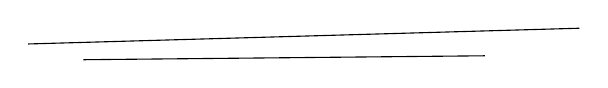
\begin{tikzpicture}
\draw (0,.2)--(7,.4);\draw (.7,0)--(5.8,.05);
\end{tikzpicture}}

\deleted{Supposons $n$ pair, $n=2m$. On s'intéresse aux systèmes
$(X,\tau_*=(\tau_i)_{0\leq i\leq n},s_0)$
\deleted{tels} non dégénérés, et tels que $\sigma(=\sigma')$ soit inv.
[Si on suppose déjà les $\beta_i$ $(0\leq i\leq n-1)$ inv.,
cela signifie $f_{\mathcal E}$ lisse.]
\deleted{Ceci définit donc}
Ceci définit donc $(X,\underbrace{Q_X}_{\text{quadrique}},\tau_*^X)$,
où maintenant les $\tau_i$ \inserted{$(0\leq i\leq n)$}
sont des autom. \unsure{involutifs} de $(X,Q_X)$.
Considérons le \unsure{antidual|multidual}:
\[
(C,Q_C,\tau_*^C)\mathbin{-}
\]
}
\mspage{54}

\scanpage{56}
Calculs \unsure{autoduaux}
\mspage{55}

\scanpage{57}
\diagram{\begin{tikzcd}[ampersand replacement=\&,column sep=small,row sep=large]
V \& a_0 \arrow[dr, no head, "1"] \& a_1 \arrow[dr, no head, "1"] \& \cdots \& a_{n-1} \arrow[dr, no head, "1"] \& a_n\\
\unsure{V'|U'} \& a'_0 \& a'_1 \& \cdots \& \& a'_n
\end{tikzcd}}
\(a'_0\) définit \(-2a_0^*+\beta_0a_1^*\).
\[
\deleted{\begin{pmatrix}
1&&&\\
-2&1&&\\
\unsure{\beta_0}&-2&1&\\
1&0&\unsure{1}&\\
\mathbin{-}&\mathbin{-}&&\\
0&0&\mathbin{-}&-2
\end{pmatrix}}
\qquad
\begin{pmatrix}
1&0&0&\mathbin{-}&\mathbin{-}&0&0&-2\\
-2&1&0&&&\big|&\big|&\beta_0\\
\beta_1&-2&1&&&\big|&\big|&0\\
0&\beta_2&-2&\diagdown&&\big|&&\big|\\
\big|&0&\beta_0&&\diagdown&\unsure{-0|0}&0&\big|\\
\big|&\big|&0&&&1&0&\\
\big|&\big|&\big|&&&\unsure{-2|\beta_{n-2}}&1&0\\
0&0&0&&&\beta_{n-2}&-2&0
\end{pmatrix}
\]
\figure{\begin{tikzpicture}
\draw (0.6,0.6) .. controls (0.3,0.3) and (-0.2,-0.1) .. (0.15,-0.15)
.. controls (0.3,-0.2) and (0.45,-0.12) .. (0.55,-0.1);
\end{tikzpicture}}
\diagram{\begin{tikzcd}[ampersand replacement=\&]
V \arrow[r,"\deleted{\unsure{\Psi}}\ \Psi"] \arrow[rr,bend left=40,"f"] \& V' \arrow[r] \& \check V\\
a_i \arrow[r,mapsto] \& \overbrace{(\beta_0\mathbin{-}\beta_{i-1})}^{c_i}a'_i
\arrow[r,mapsto] \& c_i(a_{i-1}^*\unsure{-|+}2a_i^*+\beta_i a_{i+1}^*)
\end{tikzcd}}
\[
a_1\longmapsto c_1(a_0^*\unsure{-}2a_1^*+\beta_1a_2^*)
\]
\diagram{\begin{tikzcd}[ampersand replacement=\&]
a_2\arrow[r,no head]\&c_2(a_1^*-
\end{tikzcd}}
\margin{\[
\left\{\begin{aligned}
a_0&\longmapsto a'_0\\
a_1&\longmapsto\beta_0a'_1\\
\uline{a_n}&\longmapsto(\beta_0\mathbin{-}\beta_{n-1})a'_n
\end{aligned}\right.
\qquad
\beta_0^{n\deleted{\unsure{+1}}}
\beta_1^{n-\unsure{1}}\mathbin{-}\beta_{n-1}
\]}
\[
\det\begin{pmatrix}
-2&1&0&0&\mathbin{-}&\mathbin{-}&\mathbin{-}&0&0\\
\beta_0&-2&1&0&&&&0&0\\
0&\beta_1&-2&1&&&&0&0\\
0&0&\beta_2&-2&\diagdown&&&0&0\\
0&0&0&\beta_3&\diagdown&\diagdown&&0&0\\
0&0&0&0&\diagdown&\diagdown&\diagdown&0&0\\
\big|&&&&&\diagdown&\diagdown&0&0\\
\big|&&&&&&\diagdown&0&0\\
\big|&&&&&&\diagdown&1&0\\
\big|&&&&&&\diagdown&-2&1\\
\big|&&&&&&&\beta_{n-1}&-2
\end{pmatrix}
=L_{n+1}(\beta_0\mathbin{-}\beta_{n-1})=\rho
\]
\deleted{\(\unsure{n+1}\)}
\mspage{56}

\scanpage{58}
\figure{\begin{tikzpicture}[scale=0.8]
\draw (-3.1,-0.7) -- (2.1,0.2);
\draw (-0.9,-2.2) -- (1.0,2.3);
\draw (-1.4,2.5) -- (2.0,-0.7);
\fill (-1.2,2.3) circle (2pt) node[above right] {\(h_0\)};
\fill (0.5,0.65) circle (2pt) node[above right] {\(h_1\)};
\node[above right] at (1.0,2.3) {\(H_0\)};
\node[right] at (2.1,0.2) {\(H_1\)};
\end{tikzpicture}}
\[
h_0\notin H_1\qquad \alpha=-2
\]
\deleted{
\diagram{\begin{tikzcd}[ampersand replacement=\&]h_0\arrow[r,no head]\&H_0\end{tikzcd}}
\[
\underset{\text{dernier}}{h_i}\in\deleted{\unsure{V}}L
\qquad h_j\notin L\text{ si }j>i
\]
donc \(L\subset H_j\) si \(j>i\)
\[
L\subset\underbrace{H_{i+1}\cap H_{i+2}\mathbin{-}\cap H_{n-1}}_Z
\]
\diagram{\(\begin{array}{ccc}h_0&h_1&h_2\\H_0&H_1&H_2\end{array}\)}
\deleted{\unsure{pts invariants} de \(X\)}

\unsure{Var'tés invariantes}

a) Contenu dans aucun des \(H_i\): \deleted{\(Z\)}
doit contenir les \(h_i\); c'est \(X\).

b) Contenu dans \deleted{\(\unsure{H_2}\)} un et un seul des \(H_i\)

1) Contenu dans \(H_0\), pas \(H_1,H_2\), donc \unsure{contient} \(h_1,h_2\)
il faut donc \(\uline{h_1,h_2\in H_0}\) i.e. \(\boxed{\beta_0=0}\)
on trouve \deleted{\(\unsure{H_0}\)} \(\operatorname{dr}(h_1,h_2)\)

\margin{\figure{\begin{tikzpicture}\node[draw,ellipse] {et};\end{tikzpicture}}
[\(2\beta_{\unsure{1}}\) \deleted{\unsure{pas}} mais les
\deleted{\unsure{critères}} \unsure{plus courts}
\unsure{car} \(Z\subset H_{\unsure{1}}\)]}

2) Contenu dans \(H_1\), pas en \(H_0,H_2\)
\unsure{fini}.

\[
Z\subset H_i\Rightarrow Z\subset H_{j-1}\quad\unsure{\text{avec }i\leq j}
\]
Car si \(Z\not\subset H_{j-1}\), on a \(Z\ni h_{j-1}\) donc
\(h_{i-1}\deleted{\unsure{\notin}}\in H_i\); \unsure{absurde}.
\[
Z\ni h_i\Rightarrow Z\unsure{\ni|\not\ni}h_{i+1},
\quad(\text{sinon }Z\subset H_{i+1},
\quad\text{d'où }h_i\subset
\]
\diagram{\(\begin{array}{c}
Z\subset\underbrace{H_0\cap\mathbin{-}\cap H_i}_{\dim n+1-(i+1)=n-i}\\
\cup\\
V(h_{i+1}\mathbin{-}h_{\unsure{n}})
\quad \dim (n\deleted{\unsure{+1}}-i)\unsure{-|+}1=n-i-1
\end{array}\)}
}
\mspage{57}

\scanpage{59}
\deleted{\(\langle s_0,a'_0\rangle\)}
\deleted{\(s_i,a'_i\)}
\margin{\(\unsure{\rho_{ij}|\beta_{ij}}=\unsure{\rho'_{ji}|\beta'_{ji}}:\)}
\[
\langle a_i,a'_j\rangle=
\begin{cases}
0&\text{si }j\ne i-1,i,i+1\\
1&\text{si }j=i+1\\
\mu_i=\lambda_i-1&\text{si }j=i\\
\beta_j&\text{si }j=i-1
\end{cases}
\]
\diagram{\begin{tikzcd}[ampersand replacement=\&,every matrix/.append style={name=inc,nodes in empty cells},column sep=small,row sep=large,execute at end picture={
\draw (inc-1-2.north west) .. controls +(0,0.3) and +(-0.2,0) .. (inc-1-4.north)
.. controls +(0.1,0.3) and +(-0.1,0.3) .. (inc-1-5.north)
.. controls +(0.2,0) and +(0,0.3) .. (inc-1-7.north east);
\node[above=12pt] at (inc-1-5.north) {\(V\)};
\draw (inc-2-2.south west) .. controls +(0,-0.3) and +(-0.2,0) .. (inc-2-4.south)
.. controls +(0.1,-0.3) and +(-0.1,-0.3) .. (inc-2-5.south)
.. controls +(0.2,0) and +(0,-0.3) .. (inc-2-7.south east);
\draw (inc-2-3.south west) .. controls +(0.3,-0.2) and +(-0.3,0) .. (inc-2-6.south)
.. controls +(0.1,-0.3) and +(-0.1,-0.3) .. (inc-2-7.south)
.. controls +(0.2,0) and +(-0.3,-0.1) .. (inc-2-8.south east);
\node[below=16pt] at (inc-2-6.south) {\(\deleted{\unsure{V'}}\)};
}]
a_{-1}\arrow[dr,no head,"1"']\&
a_0\arrow[d,no head,"\lambda_0-1"]\arrow[dr,no head,"1"]\&
a_1^{\unsure{2}}\arrow[d,no head,"\lambda_1-1"]\arrow[dr,no head,"1"]\&
a_2\arrow[d,no head,"\lambda_2-1"]\&\&
a_{n-1}\arrow[d,no head,"\lambda_{n-1}-1"]\arrow[dr,no head,"1"]\&
a_n\arrow[d,no head,"\lambda_n-1"]\arrow[dr,no head,"1"]\&\\
\&a'_0\&a'_1\&a'_2\&\&a'_{n-1}\&a'_n\&a'_{n+1}
\end{tikzcd}}
\margin{\diagram{\begin{tikzcd}[ampersand replacement=\&,every matrix/.append style={name=bs,nodes in empty cells},row sep=large,execute at end picture={
\draw (bs-2-2.south west) .. controls +(0.2,-0.25) and +(-0.2,-0.25) .. (bs-2-3.south)
.. controls +(0.2,-0.25) and +(-0.2,-0.25) .. (bs-2-4.south east);
}]
b_0\arrow[d,no head,"1"']\&b_1\arrow[d,no head,"1"]\&b_n\arrow[d,no head]\&b_{n+1}\arrow[d,no head,"1"]\\
\unsure{b'_0|a'_0}\&\unsure{b'_1|a'_1}\&b'_n\&\unsure{b'_{n+1}|a'_{n+1}}
\end{tikzcd}}}
\margin{\[
\mathcal E\supset V\qquad \mathcal E'\supset V'
\]
\diagram{\begin{tikzcd}[ampersand replacement=\&]\mathcal O_S\arrow[r]\&\mathcal E\arrow[r]\&\mathcal O_S\end{tikzcd}}}
\diagram{\begin{tikzcd}[ampersand replacement=\&,column sep=small,row sep=large]
a_{-1}\&a_0\&a_1\&a_2\& \&a_{n-1}\&a_n\& \&\\
\&a'_0\arrow[ur,no head,"\beta_0"]\&
a'_1\arrow[ur,no head,"\beta_1"]\&\&\ddots\&
a'_{n-1}\arrow[ur,no head,"\beta_{n-1}"]\&
a'_n\ \deleted{\unsure{0}}\&\&a'_{n+1}
\end{tikzcd}}
\[
V\simeq\mathcal O_S^{n+1}\qquad V'\simeq\mathcal O_S^{n+1}
\]
\diagram{\(\begin{array}{ccccc}
b_0&b_1&\mathbin{-}&b_{n+2}\\
b'&&\mathbin{-}&b'_0
\end{array}\)}
\mspage{58}

\scanpage{60}
\begin{center}
U N I V E R S I T E\\
DES SCIENCES ET TECHNIQUES\\
DU LANGUEDOC\\
-{}-{}-{}-{}-{}-{}-{}-{}-{}-{}-{}-\\
Service de la Scolarité\\
MR/GJ\\
Diffusion : Liste A\\
N\textdegree: 4001
\end{center}
Montpellier, le 26 Juin 1978

\begin{center}
\uline{AVIS DE SOUTENANCE D'UNE THESE DE DOCTORAT DE 3ème CYCLE}

\uline{( BIOCHIMIE )}
\end{center}

\uline{Nom et prénom du candidat} : BLAAS Dieter

\uline{Titre de la thèse} : Mise en évidence, caractérisation et purification partielle
d'une protéine kinase associée au virus MSV - MuLV.

\uline{Date, heure et lieu de soutenance prévus} :

5 JUILLET 1978 à 14 heures 30mn

Salle de cours n\textdegree\ 6, U. S. T. L.

\uline{Nom du Directeur de thèse} :

Monsieur le Professeur Ph. JEANTEUR.

\uline{Désignation du laboratoire où la thèse est préparée} :

Laboratoire de Biochimie Centre Paul Lamarque.

\uline{Analyse de l'ouvrage} :

Mise en évidence d'une protéine kinase associée au noyau viral
du virus oncogène à ARN, détermination de certains paramètres enzymologiques et
techniques d'isolement .

\uline{Durée approximative des recherches ayant abouti à la thèse} : 2 ans

\uline{Composition du jury proposé} :

\diagram{\(\begin{array}{lll}
\text{MM.}&:&\\
&&\text{Ph. JEANTEUR}\\
&&\text{B. LEBLEU}\\
&&\text{CJ LARSEN}\\
&&\text{J. DEMAILLE}
\end{array}\)}

Le Secrétaire Général,

\figure{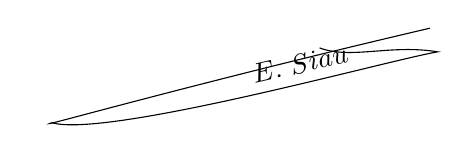
\begin{tikzpicture}
\draw (-2.7,-0.7) .. controls (-3,-0.8) and (-0.9,-0.2) .. (2.1,0.5);
\draw (-2.7,-0.7) .. controls (-2,-0.9) and (1.6,0.1) .. (2.2,0.2)
.. controls (1.6,0.3) and (1.1,0.1) .. (0.7,0.25);
\node[rotate=13] at (0.45,0.05) {\(\unsure{E.\ Siau}\)};
\end{tikzpicture}}

\uline{E. SIAU}
\mspage{59}

\scanpage{61}
\[
0\leq i\leq j\leq n-1\qquad
\rho_{ij}=L_{j-i+2}(\beta_i,\beta_{i+1},\ldots,\beta_j)
=L_{\unsure{j-i+1}}(\beta_j,\beta_{j-1},\ldots,\beta_i)
\]
\margin{\deleted{\(\widetilde\rho_{ij}=\frac12\rho_{ij}\)}}
\deleted{\(\unsure{a}\)}
\[
\rho=\rho_{0,n-1},\quad \sigma=\rho_{1,n-1},\quad
\sigma'=\rho_{0,n-2},\quad \gamma=\rho_{1,n-2}
\]
On pose aussi \(\rho_{i,i-1}=2,\quad\rho_{i,i-2}=1\)
\margin{\(\rho'_{ji}=\rho_{ij}\quad(j\geq i\)}
\[
\boxed{a_i^*=a'_{i+1}+2a'_{i+2}
+\cdots\rho_{i+1,i+j}a'_{i+j+2}+\cdots+\rho_{i+1,n-1}a'_{n+1}}
\qquad -1\unsure{\leq|<}i\leq n
\]
\deleted{\(a_j^*=\)}
en particulier pour \(i=-1,\ i=0\)
\[
\left\{\begin{aligned}
a_{-1}^*&=\Pi'=a'_0+2a'_1+
\overbrace{\rho_{0,0}}^{4-\beta_0=2-\alpha_0}a'_2+
\rho_{0,1}a'_3+\cdots+
\overbrace{\rho_{0,n-2}}^{\sigma'}a'_n+
\overbrace{\rho_{0,n-1}}^\rho a'_{n+1}\\
a_0^*&=-\Psi(a_{-1})=-\Psi(s_0)
=a'_1+2a'_2+\rho_{1,1}a'_3+\cdots+
\overbrace{\rho_{1,n-2}}^\gamma a'_n+
\overbrace{\rho_{1,n-1}}^\sigma a'_{n+1}\\
[\,a_1^*&=a'_2+2a'_3+\rho_{22}a'_{\unsure{3|4}}+\mathbin{-}
+\rho_{2,n-2}a'_n+\rho_{2,n-1}a'_{n+1}\\
&\mathbin{-}\mathbin{-}\\
a_{n-2}^*&=a'_{n-1}+2\unsure{a_n|a'_n}+
\overbrace{\rho_{n-1,n-1}}^{4-\beta_{n-1}=2-\alpha_{n-1}}a'_{n+1}\\
a_{n-1}^*&=a'_n+2a'_{n+1}\\
a_n^*&=a'_{n+1}
\end{aligned}\right.
\]
\figure{\begin{tikzpicture}
\draw[->] (0,0) .. controls (1,0.2) and (3,0.3) .. (3.6,0.1)
.. controls (4,0.2) and (4,3.2) .. (4,5.6);
\end{tikzpicture}}
\figure{\begin{tikzpicture}
\node[draw,ellipse,inner sep=12pt] {\(
\widetilde\rho_{ij}=
\begin{cases}
\deleted{\unsure{2}}\rho_{ij}&\text{si }j-i\ \deleted{\unsure{\text{impair}}}\text{pair}\\
\frac12\rho_{ij}&\text{si }j-i\ \deleted{\text{pair}}\inserted{\text{impair}}
\end{cases}\)};
\end{tikzpicture}}
\deleted{Dualement}
\[
\boxed{
a_j'^*=a_{j-1}^*+2a_{j-2}^*
+\rho'_{j-2,j-2}a_{j-3}^*+\mathbin{-}
+\rho'_{j-2,j-\unsure{i}}a_{j-\unsure{i}-1}^*
+\mathbin{-}+\rho'_{j-2,0}a_{-1}}
\]
\[
\left\{\begin{aligned}
a_{n+1}'^*&=\Pi=a_n+2a_{n-1}
+\underbrace{\rho'_{n-1,n-1}}_{4-\beta_{n-1}=2-\alpha_{n-1}}a_{n-2}
\mathbin{-}+
\overbrace{\rho'_{n-1,1}}^\sigma a_0+
\overbrace{\rho'_{n-1,0}}^\rho a_{-1}\\
a_n'^*&=-\Psi'(a'_{n+1})=a_{n-1}+2a_{n-2}
+\underbrace{\rho'_{\unsure{n-1|n-2},n-2}}_{4-\beta_{n-2}=2-\alpha_{n-2}}a_{n-3}
+\mathbin{-}+
\overbrace{\rho'_{n-2,1}}^\gamma a_0+
\overbrace{\rho'_{n-2,0}}^{\sigma'}a_{-1}\\
&\mathbin{-}\mathbin{-}\\
a_2'^*&=a_1^*+2a_{\unsure{2|0}}+
\underbrace{\rho'_{0,0}}_{4-\beta_0=2-\alpha_0}a_{-1}\\
a_1'^*&=a_0+2a_{-1}\\
a_0'^*&=a_{-1}
\end{aligned}\right.
\qquad \boxed{\langle\Pi,\Pi'\rangle=\rho}
\]
\figure{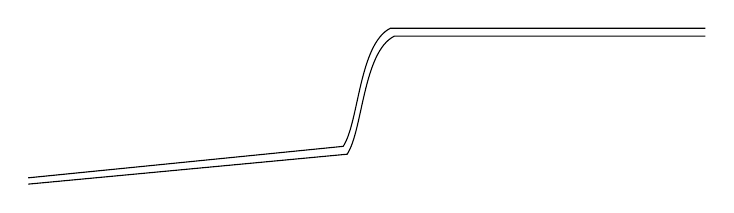
\begin{tikzpicture}
\draw (0,0)--(4,0.4).. controls (4.2,0.7) and (4.2,1.7)..(4.6,1.9)--(8.6,1.9);
\draw (0,-0.08)--(4.05,0.3).. controls (4.25,0.6) and (4.25,1.6)..(4.65,1.8)--(8.6,1.8);
\end{tikzpicture}}
\[
\left\{\begin{aligned}
\Psi(a_i)&=-(\beta_0\mathbin{-}\beta_{i-1})a'_i
&&0\leq i\leq n\\
\Psi(a_{-1})&=-a_0^*\unsure{=-|=}
[a'_1+2a'_2+\rho_{11}a'_3+\mathbin{-}\mathbin{-}
+\overbrace{\rho_{1,n-2}}^\gamma a'_n+
\overbrace{\rho_{1,n-1}}^\sigma a'_{n+1}]\\
f(a_i)&=\beta_0\mathbin{-}\beta_{i-1}&&0\leq i\leq n\\
f(a_{-1})&=0
\end{aligned}\right.
\]
\margin{\[
f(a_0)=1,\quad f(a_1)=\beta_0,\mathbin{-},\quad
f(a_n)=\beta_0\mathbin{-}\beta_{n-1}=\unsure{B|\beta}
\]}
\[
\varphi(a_i,a_{i+1})=-\deleted{\unsure{\beta_0\times}}\beta_0\mathbin{-}\beta_i
\qquad0\leq i\leq n-1
\]
\[
\Psi(\Pi)=-\sigma\Pi'\qquad
f(\Pi)=-\widetilde\sigma\widetilde\rho
\]
\mspage{60}
\mspage{60}

\scanpage{62}
\begin{center}
U N I V E R S I T E\\
DES SCIENCES ET TECHNIQUES\\
DU LANGUEDOC\\
-{}-{}-{}-{}-{}-{}-{}-{}-{}-{}-{}-\\
Service de la Scolarité\\
MR / GJ\\
Diffusion : Liste A\\
N\textdegree\ : 4151
\end{center}
Montpellier, le 1er Juillet 1978

\begin{center}
\uline{AVIS DE SOUTENANCE D'UNE THESE DE DOCTORAT DE 3ème CYCLE}

\uline{(PHYSIQUE DU SOLIDE - APPLICATION A L'ELECTRONIQUE )}
\end{center}

\uline{Nom et prénom de la candidate} : MERLET née BERNARD Catherine

\uline{Titre de la thèse} : Le phénomène de gel magnétique dans InSb : étude en fonction
du dopage.

\uline{Date, heure et lieu de soutenance prévus} :

12 JUILLET 1978 à 15 Heures,

Salle de Séminaire du C.E.E.S.- U.S.T.L.

\uline{Nom du Directeur de thèse} :

Monsieur le Professeur ROBERT.

\uline{Désignation du laboratoire où la thèse est préparée} :

Centre d'Etudes d'Electronique des Solides, MONTPELLIER.

\uline{Analyse de l'ouvrage} :

L'étude du phénomène de gel magnétique a été
faite sur des échantillons d'InSb différemment dopés (\(10^{14}\)à \(10^{16}\mathrm{cm}^{-3}\)). Ce
phénomène se traduit par une variation de l'énergie de liaison en fonction du
dopage. Pour les échantillons faiblement dopés on a mis en évidence la localisa-\\
tion d'une partie des porteurs de la bande de conduction à faible température.

\uline{Durée approximative des recherches ayant abouti à la thèse} : Deux ans

\uline{Composition du jury proposé} :

\diagram{\(\begin{array}{lll}
\text{MM.}&:&\\
&&\text{PISTOULET, Président}\\
&&\text{ROBERT}\\
&&\text{RAYMOND}\\
&&\text{LEROUX HUGON}\\
&&\text{THUILLIER}
\end{array}\)}

Le Secrétaire Général,

\figure{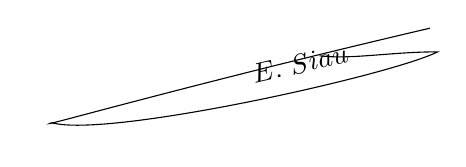
\begin{tikzpicture}
\draw (-2.7,-0.7) .. controls (-3,-0.8) and (-0.9,-0.2) .. (2.1,0.5);
\draw (-2.7,-0.7) .. controls (-2,-0.9) and (1.6,-0.1) .. (2.2,0.2)
.. controls (1.6,0.2) and (1.1,0.1) .. (0.7,0.15);
\node[rotate=13] at (0.45,0.05) {\(\unsure{E.\ Siau}\)};
\end{tikzpicture}}

\uline{E. SIAU}
\mspage{61}

\scanpage{63}
\[
\left\{\begin{aligned}
\Psi'(a'_j)&=-(\beta_{n-1}\mathbin{-}\beta_j)a_j
&&\deleted{\unsure{n+1\geq j\geq0}}\ \inserted{(n\geq j\geq0)}
\ \deleted{\unsure{-1\leq j\leq n+1}}\\
\Psi'(a'_{n+1})&=-a_n'^*
=-[a_{n-1}+2a_{n-2}+
\overbrace{\rho'_{\unsure{n-1|n-2},n-2}}^{4-\beta_{n-2}=2-\alpha_{n-2}}
+\mathbin{-}\mathbin{-}+
\overbrace{\rho'_{n-2,1}}^\gamma a_0+
\overbrace{\rho'_{n-2,0}}^{\sigma'}a_{-1}\\
f'(a'_j)&=\beta_{n-1}\mathbin{-}\beta_j
&&(n\geq j\geq\deleted{\unsure{j}}0\\
f'(a'_{n+1})&=0
\end{aligned}\right.
\]
\margin{\[
f'(a'_n)=1,\quad f'(a'_{n-1})=\beta_{n-1},
\mathbin{-},\quad
f'(a'_0)=\beta_{n-1}\mathbin{-}\beta_0=\beta
\]}
\[
\Psi'(\Pi')=-\sigma'\Pi,\qquad f'(\Pi')=-\widetilde{\sigma'}\widetilde\rho
\]
\figure{\begin{tikzpicture}\draw (0,0)--(12,0);\end{tikzpicture}}
\[
\left\{\begin{aligned}
\Psi'\Psi(a_i)&=\beta a_i&&0\leq i\leq n\\
\Psi'\Psi(\Pi)&=\sigma\sigma'\Pi
\end{aligned}\right.
\qquad(\beta=\beta_0\mathbin{-}\beta_{n-1})
\]
\[
\Psi'\Psi=\beta\operatorname{id}_{\mathcal E}+\gamma\Pi'\otimes\Pi
\qquad \boxed{\sigma\sigma'=\beta+\gamma\rho}
\]
\[
\Psi\Psi'=\beta\operatorname{id}_{\mathcal E'}+\gamma\Pi\otimes\Pi'
\]
\figure{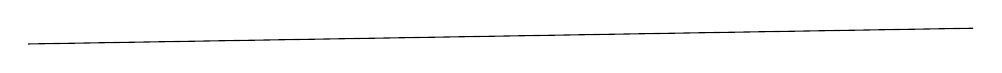
\begin{tikzpicture}\draw (0,0)--(12,0.2);\end{tikzpicture}}
\deleted{
\[
a_{-1}=s_0,\quad a'_{n+1}=s'_0
\]
\deleted{\(a_n'^*=t_0-\Psi'(a'_{n+1})=\)}
\deleted{\(a'_{n+1}=\)}
\margin{\[
\left[\begin{aligned}
s_0&=a_{-1},\\
s_1&=\tau_0s_0=s_0+a_0=a_{-1}+a_0\\
s_2&=\tau_1\tau_0s_0=s_0+(a_0+a_1)
=a_{-1}+a_0-a_1\\
&\mathbin{-}\\
s_{n+1}&=(\tau_n\mathbin{-}\tau_0)s_0
=s_0+(a_0\mathbin{-}+a_n)=a_{-1}+a_0\mathbin{-}\mathbin{-}a_n\\
s'_{\unsure{n+1|0}}&=a'_{n+1},\\
s'_n&=\tau_ns'_0=s'_{\unsure{n+1}}+a_n\\
s'_{n-1}&=\tau_{n-1}\tau_ns_0=s'_0+a_n+a_{n-1}\\
&\mathbin{-}\mathbin{-}\\
s'_0&=\tau_0\mathbin{-}\tau_ns'_0
=s'_0+(a'_n\mathbin{-}\mathbin{-}a'_0)
\end{aligned}\right.
\quad\unsure{2}
\]}
\[
t_0\overset{\text{déf}}=
\Psi'(s'_0)=\Psi'(a'_{n+1})\deleted{\unsure{\overset{\text{déf}}=}}
=-a_n'^*
=-[a_{n-1}+a_{n-2}+(4-\beta_{\unsure{n-1|n-2}})a_{n-3}
\mathbin{-}+\gamma a_0+\sigma'a_{-1}]
\]
\(t_0\) orth. à \(\overbrace{s_0\mathbin{-}s_n}\) de :
\(a_{-1},a_0,\deleted{a}\ a_n\) ?
\[
\boxed{\langle s_i,\Pi'\rangle=1\qquad
\langle\Pi,s'_i\rangle=1\qquad0\leq i\leq n+1}
\]
\[
\begin{aligned}
\varphi(t_0,s_i)&=\langle s_i,\Psi(t_0)\rangle
=\langle s_i,\Psi\Psi'(s'_0)\rangle\\
&=\langle s_i,\beta\deleted{\unsure{a'_{n+1}}}\inserted{s'_0}
+\gamma\underbrace{\langle\Pi,s'_0\rangle}_1\Pi'\rangle
=\gamma\\
&=\deleted{\unsure{\langle\ \rangle}}
\begin{cases}
\gamma&\text{si }0\leq i\leq n\\
\beta+\gamma&\text{si }i=n+1
\end{cases}
\end{aligned}
\]
\deleted{\(0\leq i\leq n\)}
\[
\varphi(\Pi,s_i)=\langle s_i,\Psi(\Pi)\rangle
=\langle s_i,-\sigma\Pi'\rangle=-\sigma.
\]
\(\sigma t_0+\gamma\Pi\) orthogonal aux \(s_i\qquad0\leq i\leq n\)
\[
\begin{aligned}
&\gamma a_n+2\gamma a_{n-1}
+\gamma\rho'_{n-1,n-1}a_{n-2}\mathbin{-}
+\gamma\overbrace{\rho'_{n-1,1}}^\sigma a_0
+\gamma\overbrace{\rho'_{n-1,0}}^\rho a_{-1}\\
&\quad-\sigma a_{n-1}\unsure{-}\sigma a_{n-2}
\qquad-\sigma\gamma a_0-\sigma\sigma'a_{-1}\\
&\hspace{6em}\uline{0.a_0-\beta a_{-1}}
\end{aligned}
\]
}
\figure{\begin{tikzpicture}
\draw (0,0)--(4.8,0.1)..controls (5.1,0.1) and (4.9,-0.4)..(5.4,-0.4)
..controls (6,-0.4) and (6.2,-0.7)..(7.4,-0.7)--(11,-0.7);
\end{tikzpicture}}
Dén. de \(\Psi^{-1}\) est \(\beta\sigma\), et
\[
\beta\sigma\Psi^{-1}=\sigma\Psi'+\gamma\Pi\otimes\Pi
\overset{\text{déf}}=\unsure{\Theta'|\Theta}
\]
\[
\beta\sigma'\Psi'^{-1}=\sigma'\Psi+\gamma\Pi'\otimes\Pi'
\overset{\text{déf}}=\Theta
\]
\figure{\begin{tikzpicture}
\node[draw,ellipse] {\(\begin{gathered}\Theta\Psi=\beta\sigma\operatorname{id}\\
\Psi\Theta=\beta\sigma\operatorname{id}\end{gathered}\)};
\end{tikzpicture}}
\[
\Theta(\Pi')=-\beta\Pi\qquad\Theta'(\Pi)=-\beta\Pi'
\]
\mspage{62}

\scanpage{64}
\begin{center}
U N I V E R S I T E\\
DES SCIENCES ET TECHNIQUES\\
\uline{DU LANGUEDOC}\\
MR/MD
\end{center}
Diffusion : Liste A\\
n\textdegree\ 4172

Montpellier, le 3 juillet 1978

\begin{center}
AVIS DE SOUTENANCE D'UNE THESE DE DOCTORAT DE SPECIALITE

\uline{SCIENCES BIOLOGIQUES} - \uline{Mention ECOLOGIE}
\end{center}

\uline{Nom et prénom du candidat} : LIVET François

\uline{Titre de la thèse} : L'herpétofaune du nord-ouest de la Montagne Noire.
Biogéographie et écologie.

\uline{Date, heure et lieu de soutenance prévus} : Jeudi 6 juillet à 8 heures -
amphithéâtre 9

\uline{Nom du Directeur de thèse} : Monsieur J. BONS

\uline{Désignation du laboratoire où la thèse est préparée} : Laboratoire de bio-\\
géographie et écologie des vertébrés E.P.H.E.

\uline{Analyse de l'ouvrage} : Le peuplement des Amphibiens et Reptiles de la Montagne
Noire a été analysé en tenant compte des milieux qui les hébergent.
Différents indices, probabilité de présence, diversité spécifique, richesse
spécifique ont été calculés et permettent de classer les milieux naturels.
L'impact humain sur certaines espèces d'Ophidiens a pu être envisagé.

\uline{Durée approximative des recherches ayant abouti à la thèse} : 3 ans

\uline{Composition du jury} :
\diagram{\(\begin{array}{l}
\text{M. R. LEGENDRE, Président}\\
\text{M. M. GODRON}\\
\text{M. J. BONS}\\
\text{M. G. PASTEUR}
\end{array}\)}

Le Secrétaire Général,

\figure{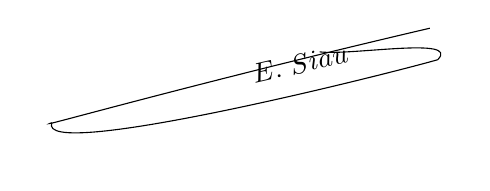
\begin{tikzpicture}
\draw (-2.7,-0.7) .. controls (-3,-0.8) and (-0.9,-0.2) .. (2.1,0.5);
\draw (-2.7,-0.7) .. controls (-2.9,-1.2) and (1.5,-0.1) .. (2.2,0.1)
.. controls (2.5,0.4) and (1.1,0.15) .. (0.7,0.2);
\node[rotate=13] at (0.45,0.05) {\(\unsure{E.\ Siau}\)};
\end{tikzpicture}}

\uline{E. SIAU}
\mspage{63}

\scanpage{65}
\[
\left\{\begin{aligned}
&s_0=a_{-1},\quad s_1=a_{-1}+a_0,\quad
s_2=a_{-1}+a_0+a_1,\mathbin{-},\quad
s_{n+1}=a_{-1}+a_0\mathbin{-}+a_n\\
&s_{i+1}=\tau_i s_i\qquad0\leq i\leq n
\end{aligned}\right.
\]
\[
\left\{\begin{aligned}
&s'_{n+1}=a'_{n+1},\quad s'_n=a'_{n+1}+a'_n,\quad
s'_{n-1}=a'_{n+1}+a'_n+a'_{n-1},\mathbin{-},\quad
s'_0=a'_{n+1}+a'_n\mathbin{-}+a'_0\\
&s'_i=\tau'_i s'_{i+1}\qquad0\leq i\leq n.
\end{aligned}\right.
\]
\[
\langle s_i,\Pi'\rangle=1\qquad\langle\Pi,s'_i\rangle=1
\]
\[
\langle s_i,s'_j\rangle=
\begin{cases}
0&\text{si }\deleted{j>i}\quad0\leq i<j\leq\unsure{n-1|n+1}\\
1&\text{si }i=j,\quad0\leq i\leq n+1
\end{cases}
\]
\[
\langle s_i,\Pi'\rangle=1\qquad
\langle\Pi,s'_j\rangle=1\qquad0\leq i\leq n+1
\]
\figure{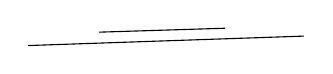
\begin{tikzpicture}
\draw (0,0)--(3.5,0.12);\draw (0.9,0.17)--(2.5,0.22);
\end{tikzpicture}}
\[
\left\{\begin{aligned}
t_i&=\Theta(s'_i)&&0\leq i\leq n+1\\
\langle t_i,\Pi\rangle&=-\beta\\
t_i&=\tau_i t_{i+1}&&0\leq i\leq n\\
\boxed{\begin{aligned}
t_{n+1}&=\Theta(s'_{n+1})=-\sigma a_n'^*+\gamma\Pi
=-\sigma a_n'^*+\gamma a_{n+1}'^*\\
&=\gamma a_n+(2\gamma-\sigma)a_{n-1}
+(\rho'_{n-1,n-1}\gamma-2\sigma)a_{n-2}+\cdots\\
&\quad+(\rho'_{n-1,n-1-j}\gamma
\deleted{\unsure{{}_{n-j}}}
-\rho'_{n-2,n-1-j}\sigma)a_{n-j-2}+\mathbin{-}\\
&\quad+(\rho'_{n-1,2}\gamma-\rho'_{n-2,2}\sigma)a_1
+\underset{!}{0.a_0}-\beta a_{-1}
\end{aligned}}
\end{aligned}\right.
\]
\[
\begin{aligned}
t_i&=t_{n+1}+\Theta(a'_n+\mathbin{-}+a'_i)\\
&=t_{n+1}-\sigma[a_n+\beta_{n-1}a_{n-1}
+\beta_{n-1}\beta_{n-2}a_{n-2}+\mathbin{-}
+(\beta_{n-1}\mathbin{-}\beta_i)a_i]
\end{aligned}
\]
\margin{\[
\Theta(a'_j)=-\sigma(\beta_{n-1}\mathbin{-}\beta_j)a_j
\qquad0\leq j\leq n
\]}
\uline{NB} \(t_i=0\) (pour \(i\) fixé) sss \(\sigma=\gamma=0\)
(et ceci implique \(\beta=0\))

Si \(\beta\) inv. (mais sans que néc. \(\sigma\) inv. i.e. \(\Psi\) iso) alors
On peut définir \(-\frac1\beta t_i\in\unsure{\overline E|E}\subset X\ \ldots\ldots\)
\[
\varphi(t_{n+1},s_i)=0\qquad0\leq i\leq n
\]
\[
\varphi(t_{n+1},a_i)=0\qquad-1\leq i\leq n-1
\]
\[
\varphi(t_{n+1},s_{n+1})=\varphi(t_{n+1},a_n)=\beta\sigma
\]
\margin{\deleted{\[
\langle t_{n+1},\Psi(a_n)\rangle
=(-2\gamma+2\gamma-\sigma)(\unsure{-\beta|\beta})=\beta\sigma
\]}
\deleted{\(=\beta a'_n\Psi t_{n+1}\)}
\[
\langle a_n,\underbrace{\Psi(t_{n+1})}_{\beta\sigma s'_{n+1}}\rangle
\]}
\[
f(t_{n+1})=\tfrac12\langle t_{n+1},
\underbrace{\Psi(t_{n+1})}_{\beta\sigma s'_{n+1}}\rangle
=\frac{\beta\sigma}{2}\gamma=\beta\widetilde\sigma\widetilde\gamma
\]
\mspage{64}

\scanpage{66}
UNIVERSITE DES SCIENCES\\
ET TECHNIQUES DU LANGUEDOC\\
\figure{\begin{tikzpicture}[x=.22cm]\draw[line width=.5pt] (0,0)--(.65,0);\draw[line width=1.2pt] (1,0)--(1.65,0);\draw[line width=1.4pt] (2,0)--(2.65,0);\draw[line width=1.2pt] (3,0)--(3.65,0);\draw[line width=.5pt] (4,0)--(4.65,0);\end{tikzpicture}}

\uline{Secrétariat Général}

Place Eugène Bataillon\\
\uuline{34060 MONTPELLIER CEDEX}

\begin{center}
\uuline{M A I\qquad1 9 7 8}

Recueil n\textdegree\ 16

\figure{\begin{tikzpicture}\draw (0,0)--(1.05,0);\end{tikzpicture}}

\uuline{CONSEIL DE L'UNIVERSITE}

\textit{Décisions prises au cours des séances}\\
\textit{des :}
\end{center}

\margin{MR LE PROFESSEUR GROTHENDIECK A.

MATHEMATIQUES\hfill5}

\diagram{\(\begin{array}{lll}
\text{= 15 Décembre 1977 (116ème séance)}&
\text{................}&\text{Conseil plénier.}\\
\text{= 12 Janvier 1978 (117ème séance)}&
\text{.................}&\text{Conseil restreint aux professeurs titulaires.}\\
\text{= 26 Janvier 1978 (118ème séance)}&
\text{.................}&\text{Conseil restreint : a) aux membres électeurs au Conseil}\\
&&\text{Scientifique}\\
&&\text{\hspace{5em}b) aux membres enseignants du Conseil}\\
\text{= 17 Février 1978 (119ème séance)}&
\text{.................}&\text{Conseil restreint aux personnels enseignants, chercheurs,}\\
&&\text{administratifs, techniques, ouvriers et de service.}\\
\text{= 3 Mars 1978 (120ème séance)}&
\text{.....................}&\text{Conseil restreint aux enseignants.}\\
\text{= 16 Mars 1978 (121ème séance)}&
\text{....................}&\text{Conseil restreint aux professeurs titulaires.}
\end{array}\)}

\begin{center}\figure{\begin{tikzpicture}\draw (0,0)--(1.05,0);\end{tikzpicture}}\end{center}
\mspage{65}

\scanpage{67}
\[
\Theta=(2-\alpha_1)\rho
\]
\deleted{
\[
\sigma\sigma'-\beta=(\underbrace{2-\alpha_1}_{(4-\beta_1)=L_2(\beta_1)=})\rho
\]
\(n=3\qquad\alpha_0,\alpha_1,\alpha_2\) paramètres
\[
\boxed{\sigma\sigma'-\beta=
\underbrace{L_{n-1}(\beta_1,\mathbin{-},\beta_{n-2})}_{\unsure{\zeta_1''|\zeta_1}=L_{n-1}(}
\rho\ \unsure{?}}
\]
\[
i:n-1
\]
\[
\Psi'\Psi=\beta\operatorname{id}+\gamma\widetilde o'\otimes\widetilde o
\qquad
\left\{\begin{aligned}
\beta&=\beta_0\beta_1\mathbin{-}\beta_{n-1}\\
\gamma&=L_{n-1}(\beta_1,\mathbin{-},\beta_{n-2})
\end{aligned}\right.
\quad ?
\]
}
\figure{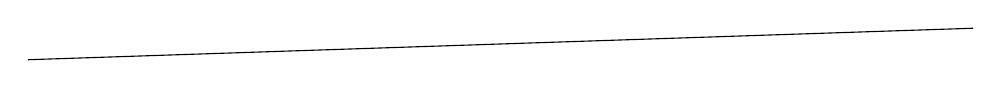
\begin{tikzpicture}\draw (0,0)--(12,0.4);\end{tikzpicture}}
\deleted{\(\unsure{\Theta}\)}
\[
\Theta(a'_{n+1})=\sigma\Psi'(a'_{n+1})+\gamma
\]
\[
\langle\underbrace{\Theta(\overbrace{a'_{n+1}}^{s'_{n+1}})}_{t_{n+1}},\Pi'\rangle
=\langle\Theta(\Pi'),\underset{a'_{n+1}}{\underbrace{s'_{n+1}}}\rangle
=-\beta\langle\Pi,s'_{n+1}\rangle=-\beta
\]
\[
u_0=s_0+s_1=2a_{-1}+a_0
\qquad\deleted{f(u)=}\langle u,\Pi\rangle=2
\]
\[
v=t_n+t_{n+1}=2t_{n+1}-\sigma a_n
\qquad\langle v,\Pi\rangle=-2\beta
\]
\[
\left\{\begin{aligned}
f(u)&=\deleted{f(s_0)+f}
4\underbrace{f(a_{-1})}_0+\underbrace{f(a_0)}_1+
2\underbrace{\varphi(a_{-1},a_0)}_{-1}=-1\\
f(v)&=\underbrace{4f(t_{n+1})}_{2\beta\sigma\gamma}
+\sigma^2\underbrace{f(a_n)}_\beta
-2\sigma\underbrace{\varphi(a_n,t_{n+1})}_{\beta\sigma}
=\beta\sigma(2\gamma-\sigma)\\
f(s_0)&=0\\
f(t_{n+1})&=\beta\widetilde\gamma\widetilde\sigma
\end{aligned}\right.
\quad\text{pour mémoire}
\]
\mspage{66}

\scanpage{68}
\begin{center}
U N I V E R S I T E\\
DES SCIENCES ET TECHNIQUES\\
DU LANGUEDOC\\
-{}-{}-{}-{}-{}-{}-{}-{}-{}-{}-{}-\\
Service de la Scolarité\\
MR / GJ\\
Diffusion : Liste A\\
N\textdegree\ :4060
\end{center}
Montpellier, le 28 Juin 1978

\begin{center}
\uline{AVIS DE SOUTENANCE D'UN DIPLOME D'ETUDES SUPERIEURES D'UNIVERSITE}
\end{center}

Le 29 JUIN 1978 à 10 Heures\\
Laboratoire de Monsieur le Professeur HALLE\\
Institut de Botanique\\
Université des Sciences et Techniques du Languedoc,

\uline{Monsieur Ibrahima DIAITE}

soutiendra un Diplôme d'Etudes Supérieures d'Université portant sur le
sujet suivant :

``Ecologie de la forêt de Basse-Casamance''.

\uline{Membres du jury}:

\diagram{\(\begin{array}{ll}
\text{MM. :}&\\
&\text{David W. LEE}\\
&\text{B. SAUGIER}\\
&\text{F. HALLE}
\end{array}\)}

Le Secrétaire Général,

\figure{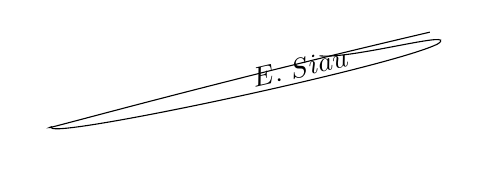
\begin{tikzpicture}
\draw (-2.7,-0.7) .. controls (-3,-0.8) and (-0.9,-0.2) .. (2.1,0.5);
\draw (-2.7,-0.7) .. controls (-2.9,-0.9) and (1.6,0.05) .. (2.2,0.35)
.. controls (2.5,0.55) and (1.1,0.15) .. (0.7,0.2);
\node[rotate=13] at (0.45,0.05) {\(\unsure{E.\ Siau}\)};
\end{tikzpicture}}

\uline{E. SIAU}
\mspage{67}

\scanpage{69}
\uline{Ex}\qquad\(\uline{n=1}\qquad\deleted{t_2=}\)
\[
\beta=\beta_0=2+\alpha,\quad\deleted{\unsure{4}}
\rho=\deleted{\unsure{\beta_0}}4-\beta=2-\alpha
\]
\[
\sigma=\sigma'=2\qquad\gamma=1
\]
\[
\left\{\begin{aligned}
\beta\sigma\Psi^{-1}&=2\beta\Psi^{-1}=2\Psi'+\Pi\otimes\Pi\\
t_2&=a_1-\beta a_{-1}\\
f(t_2)&=\beta
\end{aligned}\right.
\]

\(\uline{n=2},\quad
\beta=\beta_0\beta_1=\deleted{\unsure{\rho=}}(\alpha_0+2)(\alpha_1+2),\quad
\rho=-2(\alpha_0+\alpha_1),\quad
\sigma=2-\alpha_1,\quad\sigma'=2-\alpha_0,\quad\gamma=2\)
\margin{\deleted{\(\unsure{\alpha_0+2}\)}}
\[
\Theta=\beta\sigma\Psi^{-1}
=(4-\alpha_1^2)(\alpha_0+2)\Psi^{-1}
=(2-\alpha_1)\Psi'+2\Pi\otimes\Pi
\]
\[
t_3=2a_2+\underbrace{(2+\unsure{\alpha_1^2|\alpha_1})}_{\beta_1}a_1
+\underset{!}{0.a_0}-\beta_0\beta_1a_{-1}
\]
\[
f(t_3)=(4-\alpha_1^2)(2+\alpha_0)
\]
\mspage{68}

\scanpage{70}
\margin{\unsure{5|3}}

\uline{Etaient représentés} :

M. GOUT, par M. ROUZEYRE\\
Mme ROBIN, par Mme VERNET\\
M. THALER, par M. ASSENMACHER\\
M. KAMENKA, par M. BERTRAND\\
M. CHATELLIER, par M. FERRATON\\
M. GIRARD, par M. LABORDE\\
M. TRIAIRE, par M. RIBES\\
M. LERNER, par M. MANI

\uline{Etaient absents ou excusés} :

M.M. CHARLES, CORRIU, LEFRANC, PIETRASANTA, BENOIST,\\
SIVADE, CHICOIX, MAGOUS, Mle JUSTRABO, Mme RUSSELLO.

\uline{Assistaient à la réunion, en qualité de Directeur d'U.E.R.} :

M.M. BRUN, CANO, DURANTE, VIALLEFONT.

\uline{SITUATION DE L'U.S.T.L.}

\uline{Présidence de l'Université}

L'absence de candidature à la présidence de l'Université amène à un échange de vues auquel participent un certain nombre de membres du Conseil.

Les statuts de l'U.S.T.L. prévoyant la nécessité d'être membre du \unsure{Con}\\
pour faire acte de candidature à la présidence, le Conseil admet que la \unsure{démissio}\\
de certains membres permettrait à de nouveaux élus d'entrer au Conseil. Parmi \unsure{ce}\\
nouveaux membres certaines candidatures pourraient alors se manifester.

\uline{Commissions de spécialistes}

La motion suivante est adoptée à l'unanimité par le Conseil :

``Le Conseil de l'Université des Sciences et Techniques du Languedoc exprime le désir qu'un débat soit instauré en son sein, sur la situation créée par la mise en place de nouvelles Commissions de spécialistes''.

\figure{\begin{tikzpicture}\draw (0,0)--(14,0);\end{tikzpicture}}

\uline{120ème séance}\\
\uline{Vendredi 3 Mars 1978}

\uuline{CONSEIL RESTREINT AUX ENSEIGNANTS}

I. Approbation d'un procès-verbal\\
II. Commissions de spécialistes\\
III.Sécurité dans les laboratoires

\figure{\begin{tikzpicture}\draw (0,0)--(.6,0);\end{tikzpicture}}

\uline{Etaient présents} :

M.M. CORRIU, GAUFRES, GOUT, LEFRANC, MAURIN, Mme PARIS,\\
M.M. ROUZEYRE, THALER, Mme VERNET, M.M. DUCROT, FERRATON, RIBES.

\uline{Etaient représentés} :

M. AVEROUS, par M. ROUZEYRE\\
M. ASSENMACHER, par M. THALER\\
M. DUSSEAU, par M. DUCROT\\
M. PEYTAVIN, par M. RIBES

\uline{Etaient absents ou excusés} :

M.M. AMANIEU, CHARLES, PIETRASANTA, Mme ROBIN, M.M. ROUZAUD\\
BERTRAND, Mme CASSAGNE MEJEAN, M.M. LABORDE, LERNER, SIVADE.

\mspage{69}

\scanpage{71}
Supposons $\rho$ inv. donc $\unsure{\mathcal E|E}\simeq V\oplus\Delta_0$.

On définit, pour $\lambda$ inv,
\[
\deleted{\unsure{E_{\lambda}}}\quad
p_\lambda:\lambda\overline E\xrightarrow{\sim}V
\]
\diagram{\begin{tikzcd}[ampersand replacement=\&,column sep=large]
x\arrow[r,mapsto]\&\frac1\lambda x-
\tikz[baseline=(c.base)]{\node[draw,ellipse,inner sep=2pt](c){$\dfrac{\Pi}{\rho}$};}
\arrow[d,dash,bend right=30]\\
\&c\quad\text{si }\deleted{\text{\unsure{cela exist}}}
\end{tikzcd}}

Posons
\[
\widetilde s_i=p_1(s_i)=s_i-c\deleted{\unsure{=}}
\]
\[
\left\{\begin{aligned}
\widetilde s_0
&=\deleted{\unsure{-\left[\frac{\sigma}{\rho}a_0+2\right]}}
-\frac1\rho\left[
\deleted{\unsure{a_{-1}}}
\overbrace{\rho'_{n-1,1}}^{\sigma}a_0+
\rho'_{\unsure{n-1|n-2},2}a_1+\mathbin{-}+
\rho'_{n-1,n-1}a_{n-2}+2a_{n-1}+a_n\right]\\
\widetilde s_i
&=\widetilde s_0-\frac1\rho[a_0+\mathbin{-}+a_{i-1}]
\end{aligned}\right.
\]
\margin{$2$ inv}
\[
\widetilde u=p_2(\deleted{\unsure{u}}\inserted{u})
=\frac12u-c=a_{-1}+\frac12a_0-c
=\frac12(\widetilde s_0+\widetilde s_1)
=\widetilde s_0+\frac12a_0
\]
\figure{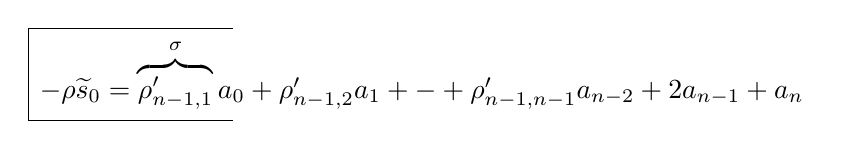
\begin{tikzpicture}
\node[anchor=west,inner sep=4pt](r) at (0,0)
{$-\rho\widetilde s_0=\overbrace{\rho'_{n-1,1}}^\sigma a_0+
\rho'_{n-1,2}a_1+\mathbin{-}+
\rho'_{n-1,n-1}a_{n-2}+2a_{n-1}+a_n$};
\draw ([xshift=2.6cm]r.north west)--(r.north west)--(r.south west)--([xshift=2.6cm]r.south west);
\end{tikzpicture}}
\figure{\begin{tikzpicture}
\node[anchor=west,inner sep=4pt](r) at (0,0)
{$\begin{aligned}
-\rho\widetilde u&=-\rho\widetilde s_0\unsure{-|+}\widetilde\rho a_0
=(\unsure{\sigma|\rho}-\widetilde\rho)a_0+
\rho'_{n-1,2}a_1+\mathbin{-}+
\rho'_{n-1,n-1}a_{n-2}+2a_{n-1}+a_n\\
-2\rho\widetilde u&=(4\widetilde\sigma-\rho)a_0+
2\rho'_{n-1,2}a_1+\mathbin{-}+
2\rho'_{n-1,n-1}a_{n-2}+4a_{n-1}+2a_n
\end{aligned}$};
\draw ([xshift=2cm]r.north west)--(r.north west)--(r.south west)--([xshift=.4cm]r.south west);
\end{tikzpicture}}
\margin{\uline{$n$ pair}\quad$(\rho=2\widetilde\rho)$}
\margin{\unsure{Cas impair}\quad$\sigma=2\widetilde\sigma$}
\[
\widetilde t_i=p_{\unsure{\beta|-\beta}}(t_i)
=-\frac1\beta t_i-c
\]
\[
-\rho\widetilde t_i=+\frac\rho\beta t_i+\Pi
\]
\margin{\unsure{si $i\geqslant1$},
coeff. de $a_0$ est $\deleted{\unsure{4}}-1/\rho$}
\margin{coeff. de $a_n$ est
$-\frac\gamma\beta-\frac1\rho
=-\frac{\beta+\gamma\rho}{\beta\rho}
=-\frac{\sigma\sigma'}{\beta\rho}$}
\[
\begin{aligned}
\text{coeff de }a_{n-1}:\
-\frac{2\gamma-\sigma}{\beta}-\frac2\rho
&=-\frac{2\gamma\rho-\sigma\rho-2\beta}{\beta\rho}\\
&=\frac{-2\sigma\sigma'-\sigma\rho}{\beta\rho}
=-\frac{\sigma}{\beta\rho}[2\sigma'+\rho].
\end{aligned}
\]
\[
-\rho\beta\widetilde t_i=\rho t_i+\beta\Pi\deleted{\unsure{=}}
\]
\[
\begin{aligned}
-\rho\beta\widetilde t_{n+1}
&=\deleted{\rho t_{n+1}+\beta\Pi
=(\rho\gamma+\beta)a_n+
[\rho(2\gamma-\sigma)+2\beta]a_{n-1}+}\\
&\quad\deleted{\unsure{\rho\sigma a_n'{}^*+\rho\gamma\Pi}}\\
&=-\rho\sigma a_n'{}^*
+\underbrace{\rho\gamma\Pi+\beta\Pi}_{\sigma\sigma'\Pi}
\end{aligned}
\]
\margin{$\deleted{2\sigma\sigma'-\rho\sigma=\sigma(2\sigma'-\rho)}$}
\[
\deleted{t_{n+1}=\Theta s_{n+1}'}
=\sigma[\sigma'\underbrace{\Pi}_{a_{n+1}'{}^*}-\rho a_n'{}^*].
\]
\figure{\begin{tikzpicture}
\node[anchor=west,inner sep=4pt](r) at (0,0)
{$-\dfrac{\rho\beta}{\sigma}\widetilde t_{n+1}
=\sigma'a_{n+1}'{}^*-\rho a_n'{}^*=\mathbin{\cdots}$};
\draw (r.north east)--(r.north west)--(r.south west)--(r.south east);
\end{tikzpicture}}
\[
-\frac{\rho\beta}{\sigma}\widetilde t_i
=-\frac{\rho\beta}{\sigma}\widetilde t_{n+1}
+\rho\beta\left(a_n+\beta_{n-1}a_{n-1}+\mathbin{-}
+(\beta_{n-1}\cdots\beta_i)a_i\right)
\]
\mspage{70}

\scanpage{72}
Calculs centrés en $\unsure{o|c}$

(si centre à dist. finie,\\
i.e. $\rho$ inv.)

\mspage{71}

\scanpage{73}
\deleted{
\uline{Choisissons} \inserted{\uline{\unsure{loc (Zar)}}} section $s_0$ de $X$ admissible pour le syst. des $(\tau_i^X)$,
(déterminé mod homothétie dans $\overline E=X\setminus C$ muni de \uline{l'origine $c$}).

Cas $c\notin C$ en tt pt \inserted{i.e. $\rho$ inv}
($n$ impair et $\rho'$ \deleted{\unsure{iff}} inv., ou
$n$ pair \deleted{et $2$ inv} \inserted{(car $\rho=2\rho'$)})
--- \deleted{donc est} Donc on est dans les conditions suivantes
(identifions $\overline E$ à $V$ grâce à l'origine $c=0$)

a) $\varphi_G^V:G\longrightarrow
\deleted{\unsure{\operatorname{Aut}(V),\mathbf G_m}}O(f)$

b) \deleted{Section $s_0$ d} base $s_0$ de
$D_0^*=\bigcap_{1\leq i\leq n}H_i^!$
$(H_i^!=H_i\setminus H_i\cap\unsure{\overline C|C})$
}
\margin{$\unsure{a_{-1}^*}$}

On a $\boxed{\text{dans }\check V}$
\[
\begin{aligned}
a_0^\vee&=\deleted{\lambda_0-1}(\lambda_0-1)a_0^*+\beta_0a_1^*\\
a_i^\vee&=a_{i-1}^*+(\lambda_i-1)a_i^*+\beta_i a_{i+1}^*
&&1\leq i\leq n-1\\
a_n^\vee&=a_{n-1}^*+(\lambda_n-1)a_n^*
\end{aligned}
\]
\margin{\uline{NB} $\rho$ inv. \unsure{exprime} ici que, \unsure{posant}
$D_0=\bigcap_{1\leq i\leq n}H_i$,
i.e. $a_0^\vee|D_0\neq0$ sur chaque fibre
(conséquence des \unsure{deuxièmes condit$^\circ$s} dans $1^\circ$)}
\deleted{\unsure{b)\quad s_0\quad a_{-1}}}

(Attention au chgt des notations, il n'y a plus de
$a_{-1},a_{-1}^*\ \cdots$)
\[
\deleted{\unsure{a_i^\vee}}\quad
\figure{
\begin{tikzpicture}[baseline=(s.base)]\node[draw,circle,inner sep=2pt](s){$*$};\end{tikzpicture}}
\qquad
s_0=\deleted{\unsure{\frac{\sigma}{\rho}a_0+\zeta}}
\inserted{=\widetilde s_0=}
-\frac1\rho(\zeta_0a_0+\zeta_1a_1+\mathbin{-}+\zeta_n a_n)
\]
\margin{On suppose pour simplifier maintenant les $\lambda_i=-1$
($\tau_i$ \uline{réflexions})}
\[
\zeta_n=1,\qquad \zeta_{n-1}=2,\qquad
\zeta_i=L_{\unsure{n+i|n-i}}(\beta_{n-1},\ldots,\beta_{i+1})
\]
\[
\left[
\begin{aligned}
\tau_i^V(s_0)&=s_0&&1\leq i\leq n\\
\text{i.e.}\quad\langle s_0,a_i^\vee\rangle&=0&&1\leq i\leq n\\
\tau_0^Vs_0&=s_0+a_0&&\text{i.e.}\quad\langle s_0,a_0^\vee\rangle=1
\end{aligned}
\right]
\]
\[
\unsure{\overline\zeta_0|\zeta_0}
=L_n(\beta_{n-1},\ldots,\beta_1)
=L_n(\beta_1,\mathbin{-},\beta_n)=\sigma
\]

C) Formes quadratiques invariantes :
\deleted{\unsure{constituent}}\inserted{elles forment}
un \deleted{torseur} $\mathcal O_S$-Module \inserted{loc}
libre de rg $1$. On normalise par
\[
\left\{
\begin{aligned}
f_V(a_0)&=1\quad\Rightarrow\quad
f_V(a_i)=\beta_0\beta_1\mathbin{-}\beta_{i-1}\\
\varphi(a_i,a_j)&=\unsure{\{0\}|0}
\quad\text{si }i,j\text{ non consécutifs}\\
\varphi(a_i,a_{i+1})&=-\beta_0\mathbin{-}\beta_i
\end{aligned}\right.
\]
\mspage{72}

\scanpage{74}
Reformulation des données lorsque $c\notin C$ en ttes fibres
i.e. $\rho$ inv ($n$ impair, $\rho'$ inv, ou $n$ pair, $\rho'$ inv. et $2$ inv.).

A) $\varphi_G:G\longrightarrow\operatorname{Aut}(X)$
ou encore $(\tau_i^X)_{0\leq i\leq n}$

est remplacé par
\[
\varphi_G:G\longrightarrow\operatorname{Aut}(V)
\quad\text{ou encore }(\tau_i^V)_{0\leq i\leq n}
\]

Conditions

$1^\circ)$ Les $\tau_i^V$ pseudo-réflexions
\[
(\text{\unsure{déf}} \quad L_i\subset\unsure{V_i|V},\ H_i\subset\unsure{V_i|V})
\]

\margin{\deleted{\unsure{dans les fibres}}}

$2^\circ)$
\[
V=\bigoplus_{0\leq i\leq n}L_i,\quad
\check V\simeq\bigoplus\underbrace{H_i^0}_{\unsure{L'_0|L'_i}}
\quad\text{i.e. }\bigcap_{0\leq i\leq n}H_i=0
\quad\text{\unsure{ch. q. fibre}}
\]

$3^\circ)$ $L_i\subset H_{i+1}$ ch. q. fibre
\hfill$0\leq i\leq n-1$

\deleted{$4^\circ)$ Posons $D_0=\bigcap_{1\leq i\leq n}H_i$,
\unsure{i.e. le}}

B) La donnée de $s_0\in\unsure{\Gamma(X)|X}$
\deleted{$\mathbin{-}$}
donnant lieu avec $\varphi_G$ à une orb. géom non dég,
est \deleted{\unsure{un pt}} exprimée par
\[
\uline{\widetilde s_0\text{ base de}}\quad
D_0=\bigcap_{1\leq i\leq n}H_i
\]
qui épingle la situation.
\deleted{On choisit}
[Il revient au $=$ de se donner une base
\deleted{C) Les formes quadratiques}
$a'_0$ de $L'_0$ (car $D_0\otimes L'_0\xrightarrow{\sim}\mathcal O_S$, par
\[
\boxed{\langle\widetilde s_0,a'_0\rangle=1}
\]
ce qui fixe \unsure{base} $a_0$ de $L_0$ par
$\tau_0=\operatorname{id}_V+a'_0\otimes a_0$,
et de proche en proche on détermine les $a'_i,a_i$ par
\[
\langle a_i,a'_{i+1}\rangle=1,\qquad
\tau_i=\operatorname{id}+a'_i\otimes a_i
\quad]
\]
\mspage{73}

\scanpage{75}
Posant
\[
\omega_V=a_0\wedge\mathbin{-}\wedge a_n
\]
on a
\[
\delta(f_V)
=\underbrace{\beta_0^n\beta_1^{n-1}\cdots\beta_{n-1}}_B
\rho\omega_V^{\otimes-2}
=B\rho\omega_V^{\otimes-2}
\]
($f$ lisse sss $B$ inv. i.e. les $\beta_i$ inv
\quad$0\leq i\leq\unsure{1|n-1}$)

Considérons alors
\[
\lambda=f_V(\widetilde s_0)
=\deleted{\unsure{-}}\frac{\sigma'\rho'}{\rho^2}
=\left\{\begin{array}{ll}
(n\text{ pair avec }\rho=2\rho')\ (2\text{ inv!})
&+\dfrac{\sigma'}{4\rho'}\\
n\text{ impair }\rho=\rho'
&+\dfrac{\sigma'}{\rho'}
\end{array}\right.
\]

La hyperquadrique affine circonscrite au polyèdre régulier est donc donnée par
\[
f_V-\lambda=0
\]
Pour qu'elle soit \deleted{\unsure{affine}}\inserted{projectivement}
lisse il f et s. que les $\beta_i$ et $\sigma'$ soient inv
(c'est donc le cas \uline{birégulier})

(D) \uline{NB} Supposons donnés $V$, $f_V$ et $\varphi_G^V$,
représentation
\[
\deleted{\text{\unsure{orth.}}}\qquad G\longrightarrow O(f_V)
\]
$1^\circ$ transformant les $\tau_i$ en réflexions \uline{orth.}
et satisfaisant de plus $2^\circ)$ $3^\circ)$ plus haut.
\deleted{\unsure{Supposons de plus}}\inserted{Ceci implique}
\[
\deleted{\unsure{4^\circ)}}
\left[
\deleted{f|(D_0=\bigcap_{1\leq i\leq n}H_i)}
\inserted{f|L_0}\neq0\quad\text{en ttes fibres.}
\right.
\]
\margin{(i.e. $\tau_0$ est une réflexion str. orth. de $V$)
\quad$\longleftrightarrow$}
\margin{\deleted{\unsure{C}}
\unsure{Cette condition entraîne celles des autres ?}}

Alors ça provient donc \unsure{fppf} d'une \unsure{sit.} \uline{\unsure{li}}
comme plus haut. Il suffit de choisir une section \inserted{$a_0$} de $D_0$
telle que $f_V(a_0)=1$

\mspage{74}

\scanpage{76}
(L'indétermination est donc section d'un rev. principal de $S$ de groupe $\mu_2$,
défini mod él. de $\mu_2(S)\ \ldots$).
Donc $s_0$ est alors donné par la formule $(*)$.
(Rien n'empêche d'ailleurs que $f_V(s_0)=0$)

\deleted{(E) \unsure{Supposons à présent}}
Si on se donne une hom
\[
\varphi_G^C:G\mathbin{-}\operatorname{Aut}(C,Q_C)
\]
[$C$ fibré proj. de rg $n$, $Q_C$ \inserted{hyper}quadrique]
satisfaisant les conditions

$1)$ Les $\tau_i^X$ réflexions \deleted{orth}
\hfill$(0\leq i\leq n)$

\hfill i.e. $h_i\in\Gamma C$, $H_i$ hyperplans)

$2)$ Les $h_i$ engendrent $C$, les
$\bigcap_{0\leq i\leq n}H_i^{\unsure{C}}=\varnothing$

$3)$ \deleted{\unsure{H_i}}
\quad$h_i\notin H_{i+1}$\hfill$0\leq i\leq n-1$

\deleted{et $4)$ \unsure{un}
$\unsure{L_0|h_0}\notin Q_C$ en chaque fibre}

\margin{Pour $n\geq2$}
\margin{(Si $n=1$, une réflexion de $C$ donne \unsure{pour}
$C=P(W)$, \unsure{ne remonte pas} de \uline{façon unique}
en \unsure{réfl.} de $V\ldots$]}

alors loc. (et) ça provient de
$(V,f_V,(\tau_i^V))$ satisfaisant les conditions de (D),
$V$ déterm. mod $\otimes L$ ($L$ inv),
$f_V$ défini mod unité.
On utilise \unsure{$h_0$ pour rigidifier};
$L_0\subset V$, on les ``épingle'' i.e éliminer l'indét. $\otimes L$,
en \unsure{plongeant|choisissant} $L\simeq\mathcal O_S$
i.e. section $a_0$ de $L_0$.

\mspage{75}

\scanpage{77}
Et on normalise alors par $f(a_0)=1$.
On trouve : La catégorie des réal. géom. de $\unsure{\Pi_1|\Pi_n}$ non dég.
avec centre à distance finie, est équivalente à celle des triples
$(C,Q_C,\varphi_G^C)$ d'un fibré projectif de rg $n$,
d'une hyperquadrique $Q_C$ de $C$, d'une rep. de $G$ dans $(C,Q_C)$,
satisfaisant les conditions $1^\circ)$ à $3^\circ)$.

\margin{\uline{NB} $n\geq2$}

(\uline{NB} Si on ne se donne pas $Q_C$, c'est encore analogue,
mais \deleted{alors} $Q_C$ est déduit \unsure{canoniq$^t$|canonique}
comme unique hyperquadrique fixe.

\mspage{76}

\scanpage{78}
\margin{$\widetilde s_0=s_0-o$}
\margin{\deleted{$s'_0=\rho\widetilde s_0$\\$f_V(s'_0)$}}
\[
\begin{aligned}
f_V(\widetilde s_0)
&=f_{\unsure{E|V}}(s_0-o)
=\underbrace{f(s_0)}_0+
\underbrace{f(o)}_{-\frac{\sigma'\rho'}{\rho^2}}
-\underbrace{\varphi(s_0,o)}_{-\frac{\sigma}{\rho}}\\
&=-\frac{\sigma'\rho'}{\rho^2}+\frac{\sigma}{\rho}
\end{aligned}
\]
\[
\left\{\begin{array}{ll}
n\text{ pair }\rho=2\rho',\ \sigma^{\unsure{2|*}}=\sigma'
&
f_V(\widetilde s_0)=-\frac14\frac{\sigma'}{\rho'}
+\frac12\frac{\sigma'}{\rho'}=\frac14\frac{\sigma'}{\rho'}\\
n\text{ impair }\rho=\rho',\ \sigma=2\sigma'
&
f_V(\widetilde s_0)=-\frac{\sigma'}{\rho'}
+2\frac{\sigma'}{\rho'}=\frac{\sigma'}{\rho'}
\end{array}\right.
\]

Soit
\[
s'_0=-\rho\widetilde s_0=
\deleted{\unsure{n}}
(\underset{\sigma}{\underbrace{\zeta_0}}a_0+
\zeta_1a_1+\mathbin{-}+
\underset{1}{\underbrace{\zeta_n}}a_n)
\]
\[
f_V(s'_0)=\rho\sigma-\rho'\sigma'=\rho'\sigma'
\]
\[
\boxed{f_V(s'_0)=\rho'\sigma'}
\]
\[
\begin{aligned}
\varphi_V(\widetilde s_0,a_i)
&=\varphi_{\unsure{E|V}}(s_0-o,a_i)\\
&=\underbrace{\varphi(s_0,a_i)}_{\substack{0\text{ si }i\neq0\\-1\text{ si }i=0}}
-\underbrace{\varphi(o,a_i)}_{0\ \forall i}\\
&=\begin{cases}-1&i=0\\0&1\leq i\leq n\end{cases}
\end{aligned}
\]
\[
\left\{\begin{aligned}
\widetilde s_i&=s_i-o\\
s'_i&=-\rho\widetilde s_i
\end{aligned}\right.
\qquad
\left\{\begin{aligned}
\widetilde s_i&=\tau_{i-1}^V\widetilde s_{i-1}
\quad(1\leq i\leq n)\\
s'_i&=\tau_{i-1}^Vs'_{i-1}
\end{aligned}\right.
\]
\margin{$
\varphi_V(s'_0,a_i)=
\begin{cases}\rho&i=0\\0&1\leq i\leq n.\end{cases}
$}
\[
\left\{\begin{aligned}
\widetilde s_i&=(s_i-s_0)+(s_0-o)
=\widetilde s_0+(a_0+\mathbin{-}+a_{i-1})\\
s'_i&=s'_0\unsure{-|+}\rho(a_0+\mathbin{-}+a_{i-1})
\end{aligned}\right.
\]
\margin{
\figure{\begin{tikzpicture}
\node[anchor=west,inner sep=4pt](r)at(0,0)
{$\begin{aligned}
\langle\widetilde s_0,a_i^\vee\rangle
&=\langle\widetilde s_0,a'_i\rangle=\\
\langle s_0-o,a'_i\rangle
&=\langle s_0,a'_i\rangle\\
&=\begin{cases}1&i=0\\0&1\leq i\leq n\end{cases}
\end{aligned}$};
\draw (r.north west)--([xshift=-4pt]r.north west)--([xshift=-4pt]r.south west)--([xshift=1cm]r.south west);
\end{tikzpicture}}
}
\[
s'_1=s'_0-\rho a_0
\]
\[
\deleted{\unsure{f}}\quad s'_0+s'_1=2s'_0-\rho a_0
\]
\[
\begin{aligned}
f_V(s'_0\unsure{+|-}s'_1)
&=4\underbrace{f_V(s'_0)}_{\rho'\sigma'}
+\rho^2\underbrace{f_V(a_0)}_1
\unsure{-|+}2\rho\underbrace{\varphi_V(s'_0,a_0)}_\rho\\
&=4\rho'\sigma'-\rho^2=
\end{aligned}
\]
\[
f_V(s'_0\unsure{-|+}s'_1)=
\begin{cases}
n\text{ pair}:&4\rho'(\sigma'-\rho')\\
n\text{ impair}:&\rho'(4\sigma'-\rho')
\end{cases}
\]

Donc pour que l'homothétie de rapport $\lambda$ transforme la sphère
$\Sigma$ circonscrite aux $s'_i$ en celle circonscrite aux transformés des
$s'_0+s'_1$, il f et s. que
\[
\lambda^2\rho'\sigma'
=\deleted{\rho'(4\sigma'-\rho')}
\left\{\begin{array}{l}
4\rho'(\sigma'-\rho')\\
\deleted{\text{i.e. }\lambda=}\\
\rho'(4\sigma'-\rho')
\end{array}\right.
\]
\[
\begin{array}{lll}
\text{i.e.}&\lambda=2\sqrt{1-\rho'/\sigma'}&n\text{ pair}\\
&\lambda=2\sqrt{1-\rho'/4\sigma'}&n\text{ impair}
\end{array}
\]
\mspage{77}

\scanpage{79}

\margin{Sous-espaces invariants}

\mspage{78}

\scanpage{80}

On suppose qu'on est sur \uline{corps $k$}.

\margin{\deleted{$\unsure{a_i}$}}

\uline{Théorème} Soit $Z\subset X$ sous-espace projectif. Pour que $Z$ soit invariant par $G$ i.e. par les $\tau_i$ \inserted{$(0\leq i\leq n)$}, il \unsure{f et s.} qu'on soit dans l'un des cas suivants :

a) $Z$ est égal à l'un des s-espaces $\varnothing,X,\{c\},C$.

b) $\exists\ 0\leq i\leq n-1$ tel que $\beta_i$ \unsure{(ou $2+\alpha_i$)|(ou le $\alpha_i$)} $=0$, et on a
\[
Z=\underbrace{H_0\cap H_1\cap\cdots\cap H_i}_{Z_i'\ (\text{de dim }n-i)}
\quad\text{ou}\quad
Z=\deleted{\unsure{\mathbf P}}\underbrace{\operatorname{Lin}(h_{i+1},\ldots,h_n)}_{\substack{Z_i^{\unsure{\sharp|!}}\\(\dim n-i-1)}}.
\]
\margin{$\mathrm{NB}\quad\beta_i=0\quad\Longleftrightarrow\quad
\underbrace{Z_i\subset Z_i'}_{\text{codim }1}$.}
\margin{\unsure{b}}

(\uline{NB} On posera
\[
Z_n=\underbrace{H_0\cap\cdots\cap H_n}_{\{c\}}
\quad\text{et}\quad Z_n'=\varnothing\unsure{-\mathrm{th}.}
\]
\[
Z_{-\unsure{1}}=X\qquad Z_{-\unsure{1}}'=C
\]

On a (sans hyp. sur aucun des $\beta_i$)

\diagram{\begin{tikzcd}[ampersand replacement=\&,column sep=small,row sep=large]
Z_n^{\unsure{\sharp|!}}=\varnothing \arrow[r,phantom,"\subset"] \arrow[d,phantom,"\subset",sloped]
\& Z_{n-1}^{\unsure{\sharp|!}}=\{h_n\} \arrow[r,phantom,"\subset"] \arrow[d,phantom,"\subset",sloped]
\& Z_{n-2}^{\unsure{\sharp|!}}=\unsure{\operatorname{L}}\!(h_n,h_{n-1}) \arrow[r,phantom,"\cdots"] \arrow[d,phantom,"\subset",sloped]
\& Z_0^{\unsure{\sharp|!}}=\operatorname{L}(h_n\ldots h_1) \arrow[r,phantom,"\subset"] \arrow[d,phantom,"\subset",sloped]
\& Z_{-1}^{\unsure{\sharp|!}}=C \arrow[d,phantom,"\subset",sloped]\\
Z_n'=\{c\}\arrow[r,phantom,"\subset"]
\&Z_{n-1}'=H_0\cap\cdots\cap H_{n-1}\arrow[r,phantom,"\subset"]
\&Z_{n-2}'=H_0\cap\cdots\cap H_{n-2}\arrow[r,phantom,"\cdots"]
\&Z_0'=H_0\arrow[r,phantom,"\subset"]
\&Z_{-1}'=X
\end{tikzcd}}

Toutes les inclusions \unsure{écrites} sont strictes, de codim 1.
\deleted{Tous} les $2(n+2)$ espaces $Z_i,Z_i'$ $(-1\leq i\leq n)$ sont ils distincts ? Pour une dim donnée $-1\leq d\leq n+1$, il y a \deleted{au \unsure{plus}} \inserted{un} seul des $Z_i,Z_i'$ de cette dim si $d=-1$ ou $d=n+1$ (savoir $Z_n^{\unsure{\sharp|!}}$ et $Z_{-1}'$), et \inserted{exactement} deux si $0\leq d\leq n$, savoir
\[
Z_{n-d}'=H_0\cap\cdots\cap H_{n-d}
\quad\deleted{(\unsure{d})}
\]
et $Z_{n-d-1}^{\unsure{\sharp|!}}=\operatorname{Lin}(h_n,\ldots,h_{n-d})$, et ils \deleted{en} sont \deleted{\unsure{codim}} égaux sss $h_{n-d},h_{n-d+1}\in Z_{n-d}'$, i.e.
\[
h_{n-d}\in H_{n-d}\cap H_{n-d-1}
\qquad
h_{n-d+1}\in H_{n-d}.
\]
\margin{\uline{NB} Si $c\notin C$ i.e. $\rho\neq0$, alors les $Z_i,Z_i'$ tous distincts, $Z_i'\not\subset Z_j^{\unsure{\sharp|!}}$ pour \unsure{$\forall i,j$}.}

\mspage{79}

\scanpage{81}

i.e. sss on a simultanément (posant $i=n-d$)
\[
\left\{
\begin{array}{ll}
\mu_i\ (= \lambda_i-1)=0&
\text{(i.e. }2\cdot1_k=0\text{ dans le cas des réflexions }\unsure{\Rightarrow}\text{ i.e. }k\text{ de car. }2)\\
\beta_i=\beta_{i-1}=0&
\text{(se réduit à la condition }\beta_i=0\text{ si }i=0,\text{ et à la condition }\beta_{i-1}=0\text{ si }i=n)
\end{array}\right.
\]

\deleted{\uline{Cor} \unsure{Il y a}}
\deleted{\uline{Dém.}}

\uline{Cor.} \textcircled{a} Il y a au plus $2(n+2)$ sous-espaces projectifs invariants par $G$. \textcircled{b} Pour qu'il y en ait $2(n+2)$, il f et s. que $\beta_i=0$ $(0\leq i\leq n-1)$ et $\mu_i\neq0$ \deleted{$\unsure{\forall i}$} $(0\leq i\leq n)$ (cette condition signifie aussi, dans le cas des réflexions, que $\operatorname{car.}k\neq2$).

\textcircled{c} \deleted{Pour} Il y a au moins les quatre s-espaces invariants $\varnothing,X,\{c\},C$. Pour que ce soient les seuls, il \deleted{\unsure{faut et suffit}} \inserted{suffit} que $\beta_i\neq0$ $0\leq i\leq n-1$ (ce qui implique que les $2(n+2)$ espaces $Z_i,Z_i'$ sont distincts). Il faut \inserted{et s.} que
\[
\beta_i\neq0\quad0\unsure{<|\leq}i<n-1,
\quad\text{et que}\quad
(\beta_0\deleted{\unsure{=\beta_n}}=0\Longrightarrow\mu_0=0),
\]
\[
(\beta_{n-1}=0\Longrightarrow\mu_n=0)
\]
[donc, dans le cas des réflexions, que
\[
\left\{
\begin{array}{ll}
\text{si }\operatorname{car.}k\neq2:\text{ les }\beta_i\neq0\ (0\leq i\leq n-1),
&\text{i.e. }\beta=\prod\beta_i\neq0\\
\text{si }\operatorname{car.}k=2\quad\text{les }\beta_i\neq0\text{ si }0<i<n-1.&
\end{array}
\right.
\]

\deleted{d) Pour que \deleted{la \unsure{représentation}} la représentation projective de $G$ \uline{dans $C$} soit irréductible, il f et s. que $\rho\neq0$ et les $\beta_i\neq0$, i.e. que}

\margin{\figure{\begin{tikzpicture}
\node[draw,ellipse,align=left] at (0,0) {Si $c\notin C$\\i.e. $\rho\neq0$};
\draw[->] (1.4,.25) -- (2.2,.5);
\end{tikzpicture}}}

d) Les sous-espaces projectifs stables de $C$ $\neq C$ \deleted{et}, de $\varnothing$ \deleted{et de $\{c\}$ (en le cas $c\in C$)} sont en corr. $1-1$ avec les $0\leq i\leq n-1$ tels que $\beta_i=0$, \deleted{et} \unsure{avec les} correspondants $Z_i^{\unsure{\sharp|!}}$ (\deleted{de} dim $n-1-i$). Les deux

\mspage{80}

